% ============================================================
%  hw4_submission_final.tex  --  MATH 6660, Homework 4, Problems 1-4.
%
%  RULE: nothing in this document goes beyond the class lectures.
%  Each derivation is tagged with the lecture it comes from.  Anything that
%  would go outside them is wrapped in \outside{}{} and prints as a red
%  labelled box, so it is visible in the PDF.
%
%  Build: pdflatex hw4_submission_final.tex   (twice, for cross-references)
% ============================================================
\documentclass[11pt]{article}
\usepackage[letterpaper,margin=1in]{geometry}
\usepackage[T1]{fontenc}
\usepackage{amsmath,amssymb,amsthm}
\usepackage{booktabs}
\usepackage{array}
\usepackage{graphicx}
\usepackage{caption}
\usepackage{enumitem}
\usepackage{bm}
\usepackage{tikz}
\usepackage{xcolor}
\usepackage[colorlinks=true,linkcolor={blue!45!black},pdfborder={0 0 0}]{hyperref}
\usepackage{pdfcomment}
\usepackage{xspace}
\usepackage{colortbl}
\usepackage{tcolorbox}

% ---- element colours for the assembly box (Figure fig:assembly) ------
\definecolor{elone}{HTML}{C0392B}
\definecolor{eltwo}{HTML}{CA6F1E}
\definecolor{elthree}{HTML}{1F618D}
\definecolor{elfour}{HTML}{1E8449}
\definecolor{elfive}{HTML}{7D3C98}
\definecolor{elsix}{HTML}{0097A7}
\definecolor{elseven}{HTML}{C2185B}
\definecolor{eleight}{HTML}{8D6E63}
\definecolor{elnine}{HTML}{9E9D24}
\newcommand{\en}[2]{\tikz[baseline=(c.base)]\node[circle,draw=#2,text=#2,
  inner sep=0.7pt,font=\scriptsize\bfseries](c){#1};}

% every figure and table carries a number and sits where it was written
\captionsetup{font=small,labelfont=bf,justification=justified,
              singlelinecheck=false,skip=6pt,hypcap=false}

\newcommand{\dx}{\,\mathrm{d}x}
\newcommand{\dxdy}{\,\mathrm{d}x\,\mathrm{d}y}
\newcommand{\ds}{\,\mathrm{d}s}
\newcommand{\norm}[1]{\lVert #1\rVert}
\newcommand{\abs}[1]{\lvert #1\rvert}
\newcommand{\eps}{\varepsilon}
\newcommand{\ie}{i.e.\@\xspace}
\newcommand{\eg}{e.g.\@\xspace}
\newcommand{\Om}{\Omega}
\newcommand{\dOm}{\partial\Omega}
\newcommand{\grad}{\nabla}
\newcommand{\lap}{\Delta}
\newcommand{\Iint}{\iint_{\Om}}
\newcommand{\Vsp}{V}
\newcommand{\nn}{\bm{n}}
\setlength{\parindent}{0pt}

% ---- provenance tag: which lecture a step comes from ------------------
\newcommand{\src}[1]{{\small\color{black!55}\textsf{[#1]}}}

% ---- anything outside the lectures is boxed and labelled -------------
\newcommand{\outside}[2]{%
  \par\smallskip\noindent
  \fcolorbox{red!65!black}{red!4}{%
    \parbox{0.955\linewidth}{\small
      \textbf{\color{red!65!black}NOT FROM LECTURE --- #1}\par\smallskip #2}}%
  \par\smallskip}

% ---- bullets ---------------------------------------------------------
\newlist{steps}{itemize}{1}
\setlist[steps]{label=\textbullet, leftmargin=1.25em, topsep=3pt,
                itemsep=4pt, parsep=0pt}

% ---- hover tooltips on cross-references ------------------------------
\makeatletter
\newcommand{\settip}[2]{\expandafter\gdef\csname femtip@#1\endcsname{#2}}
\newcommand{\gettip}[1]{%
  \ifcsname femtip@#1\endcsname\csname femtip@#1\endcsname\else equation \ref{#1}\fi}
\newcommand{\eqr}[1]{\pdftooltip{\eqref{#1}}{\gettip{#1}}}
\makeatother

\settip{eq:pde}{Poisson problem: minus the Laplacian of u equals f on the square, u equals g on its boundary}
\settip{eq:ibp}{After the product rule and the divergence theorem: gradient-gradient integral minus the boundary integral of v times the normal derivative equals the load integral}
\settip{eq:weak}{Weak form: the integral of grad u dot grad v equals the integral of f v}
\settip{eq:spaces}{Trial set V_g: finite energy and v equals g on the boundary. Test space V_0: finite energy and v equals 0 on the boundary}
\settip{eq:lifted}{Lifted problem: B(w,v) equals L-tilde(v) for all v in V_0, with u = w + G}
\settip{eq:poinc}{Poincare on the square: the L2 norm squared of v is at most 4 times the L2 norm squared of grad v}
\settip{eq:ke}{Element stiffness matrix of the bilinear square, one sixth of 4,-1,-2,-1 and its cyclic shifts}
\settip{eq:row}{Assembled equation for interior node (i,j): one third of 8 U_ij minus its eight neighbours equals b_ij}
\settip{eq:hatsQ}{The four corner hat functions on a square: (x_{i+1}-x) or (x-x_i) times (y_{j+1}-y) or (y-y_j), divided by h^2}
\usepackage{amsmath,amssymb}
\usepackage{fancyvrb}
\newcommand{\problem}[2]{%
  \section*{Problem #1}%
  \renewcommand{\theequation}{#2.\arabic{equation}}%
  \setcounter{equation}{0}}
\begin{document}


\begin{center}
  {\large\bfseries MATH 6660 --- Homework 4}\\[2pt]
  {\small Md Mahmudul Hasan Mollah}
\end{center}



% ==================================================================
\problem{1}{1}

\textit{Download the PyDistMesh mesh generator.  You can find all the
necessary links from the Math 6660 Canvas page.}

PyDistMesh, B.~Froehle's Python port of P.-O.~Persson's \textsc{DistMesh},
was downloaded from the Canvas page and is used unmodified in Problems 2
and 3.  Table~\ref{tab:p1files} lists the files in the package.
 

\begin{center}
\begin{minipage}{\linewidth}
\centering\footnotesize
\begin{tabular}{@{}>{\raggedright\arraybackslash}p{0.27\linewidth}>{\raggedright\arraybackslash}p{0.69\linewidth}@{}}
\toprule
file & role\\
\midrule
\texttt{distmesh2d.py} & \texttt{p,t = distmesh2d(fd,fh,h0,bbox,pfix)}: level set
  \texttt{fd}, relative size \texttt{fh}, edge length \texttt{h0}; returns
  nodes \texttt{p} ($N\times2$) and triangles \texttt{t} ($M\times3$)\\
\texttt{distance\_functions.py} & level sets (\texttt{dcircle},
  \texttt{drectangle}, \dots) and Booleans: \texttt{dunion} $=\min$,
  \texttt{dintersect} $=\max$, \texttt{ddiff}$(d_1,d_2)=\max(d_1,-d_2)$\\
\texttt{boundary.py} & \texttt{bnd2d}: re-triangulates, marks nodes with
  $\abs{\phi}\le10^{-8}$ as boundary and puts them last, returns the areas\\
\texttt{assemble.py} & the CG(1) code used in Problem 3\\
\texttt{example1.py}, \texttt{example2.py}, \texttt{poisson\_example.py} &
  unit disc; square with a hole, graded; $-\lap u=1$ on the latter\\
\bottomrule
\end{tabular}
\captionof{table}{The PyDistMesh bundle as downloaded (plus two helper files,
\texttt{utils.py} and \texttt{mlcompat.py}).}
\label{tab:p1files}
\end{minipage}
\end{center}

 


 \newpage

% ==================================================================
\problem{2}{2}

\textit{Use this code to generate a mesh for a star-shaped region whose
boundary is the zero contour of $\phi(r,\theta)=r-0.75-0.25\sin(5\theta)$.}

\subsection*{The level set in Cartesian coordinates}

PyDistMesh evaluates the level-set function \texttt{fd} at Cartesian points,
so $\phi$ is rewritten with $r=\sqrt{x^{2}+y^{2}}$ and
$\theta=\tan^{-1}(y/x)$, taken in the quadrant of the point $(x,y)$:
\begin{equation}\label{eq:phi}
  \begin{gathered}
  \phi(x,y)=\sqrt{x^{2}+y^{2}}-0.75-0.25\sin\bigl(5\tan^{-1}(y/x)\bigr),\\
  \phi<0\iff r<R(\theta):=0.75+0.25\sin5\theta .
  \end{gathered}
\end{equation}
The boundary radius $R(\theta)$ lies between $0.5$ and $1$, so the star has
five tips at $r=1$ and five valleys at $r=0.5$, and the box $(-1,1)^{2}$
contains $\Om$.  The mesh is generated by
\begin{Verbatim}[fontsize=\small,xleftmargin=1em]
fd = lambda p: np.sqrt(p[:,0]**2 + p[:,1]**2) - 0.75 \
               - 0.25*np.sin(5*np.arctan2(p[:,1], p[:,0]))
p, t = dm.distmesh2d(fd, distfunc.huniform, h0, (-1,-1,1,1))
p, t, nin, nbd, area = bnd.bnd2d(fd, p, t, -1.0, -1.0, 1.0, 1.0)
\end{Verbatim}
To check the mesh, the exact area of the star is computed in polar
coordinates:
\begin{equation}\label{eq:area}
  \abs{\Om}=\int_{0}^{2\pi}\!\!\int_{0}^{R(\theta)}r\,\mathrm{d}r\,\mathrm{d}\theta
  =\frac12\int_{0}^{2\pi}\Bigl[0.75^{2}+1.5\cdot0.25\underbrace{\sin5\theta}_{\int=\,0}
   +0.25^{2}\underbrace{\sin^{2}5\theta}_{\int=\,\pi}\Bigr]\mathrm{d}\theta
  =\frac{19\pi}{32}=1.86532 .
\end{equation}

\subsection*{The boundary nodes}

\texttt{bnd2d} marks a node as boundary only if $\abs{\phi}\le10^{-8}$, and
Problem 3 imposes $u=0$ only at those nodes.  On the star, $66$ of the $138$
nodes on boundary edges sit just inside the curve, $\phi\approx-10^{-4}$,
around the valleys (red in Figure~\ref{fig:p2}), and are missed.  Before
\texttt{bnd2d}, every node on a boundary edge is therefore moved radially
onto the curve,
\begin{equation}\label{eq:snap}
  (x,y)\;\leftarrow\;R(\theta)\,(\cos\theta,\sin\theta),
  \qquad\text{so}\quad \phi=0 ,
\end{equation}
a move of at most $10^{-4}\ll h_{0}$.  Afterwards every boundary node is
marked (Table~\ref{tab:p2}).


\subsection*{The mesh}

\begin{center}
\begin{minipage}{\linewidth}
\centering
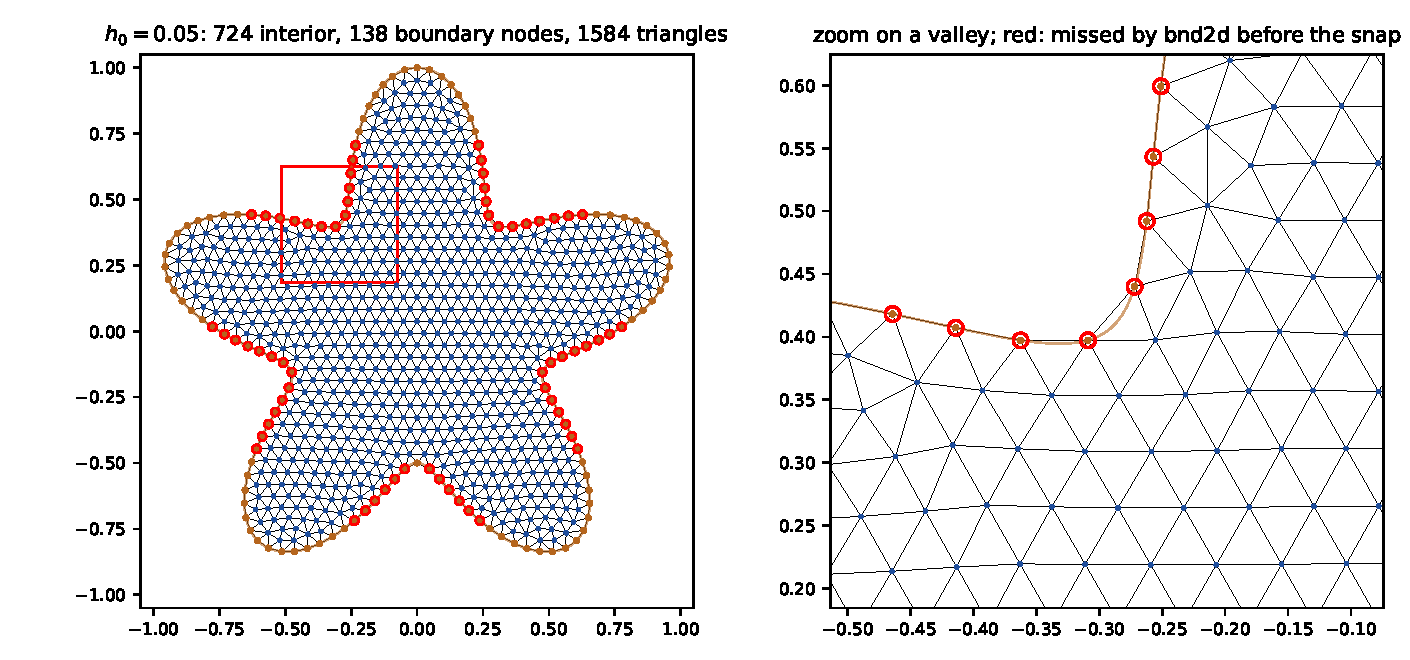
\includegraphics[width=0.97\linewidth]{hw4_p2_mesh.pdf}
\captionof{figure}{The star mesh at $h_{0}=0.05$, after the fix
\eqref{eq:snap}.  Blue: interior nodes; brown: boundary nodes; the curve is
$\phi=0$.  Red circles: the boundary nodes that \texttt{bnd2d} classed as
interior before the fix.}
\label{fig:p2}
\end{minipage}
\end{center}

\begin{center}
\begin{minipage}{\linewidth}
\centering\small\setlength{\tabcolsep}{4pt}
\begin{tabular}{@{}rrrrrrrc@{}}
\toprule
$h_0$ & interior & boundary & elements & mesh area & rel.\ error & $\max_j h_j/\rho_j$ & flagged: raw $\to$ snapped\\
\midrule
0.100 & 149 & 66 & 362 & 1.86001 & $-2.8\!\times\!10^{-3}$ & 2.57 & 32/66 $\to$ 66/66\\
0.050 & 724 & 138 & 1584 & 1.86432 & $-5.4\!\times\!10^{-4}$ & 2.46 & 72/138 $\to$ 138/138\\
0.025 & 3167 & 282 & 6614 & 1.86498 & $-1.9\!\times\!10^{-4}$ & 2.45 & 140/282 $\to$ 282/282\\
\bottomrule
\end{tabular}

\captionof{table}{Star meshes.  Exact area $19\pi/32=1.86532$
\eqref{eq:area}.  Last column: nodes \texttt{bnd2d} marks as boundary, out of
the nodes on boundary edges, before and after \eqref{eq:snap}.}
\label{tab:p2}
\end{minipage}
\end{center}

Table~\ref{tab:p2} shows the area error falling from $0.3\%$ to $0.02\%$ as
$h_{0}$ decreases from $0.1$ to $0.025$.  The ratio $\max_{j}h_{j}/\rho_{j}$
stays at or below $2.57$ on every mesh, against $1.73$ for an equilateral
triangle, so the meshes are regular in the sense of (1.260) and have no
slivers in the valleys.


\newpage
% ==================================================================
\problem{3}{3}

\textit{Use the CG(1) method developed in class and provided on the Math 6660
Canvas page to solve $-u_{,xx}-u_{,yy}=1$ in $\Om$, $u=0$ on $\dOm$, on the
star of Problem 2.}

\subsection*{The method}

Let $V=H^{1}_{0}(\Om)$.  The weak form of the problem is: find $u\in V$ such
that
\begin{equation}\label{eq:weak3}
  \iint_{\Om}\grad u\cdot\grad v\dxdy=\iint_{\Om}f v\dxdy
  \qquad\text{for all } v\in V,
\end{equation}
with $f=1$.  Let $V_{h}$ be the space of continuous functions that are linear
on each triangle of the Problem 2 mesh and vanish at the boundary nodes.  Such
functions have square-integrable gradients and vanish on the boundary, so
$V_{h}\subset V$.  (Strictly, the mesh covers a polygon that differs from
$\Om$ by slivers of width $\mathcal O(h^{2})$ along the curved boundary; this
difference is neglected.)  The CG(1) approximation $U$ is obtained by
restricting \eqref{eq:weak3} to this subspace: find $U\in V_{h}$ such that
\begin{equation}\label{eq:galerkin3}
  \iint_{\Om}\grad U\cdot\grad v\dxdy=\iint_{\Om}f v\dxdy
  \qquad\text{for all } v\in V_{h}.
\end{equation}
A basis of $V_{h}$ is formed by the hat functions $\varphi_{1},\dots,\varphi_{M}$
of the $M$ interior nodes.  Writing $U=\sum_{i=1}^{M}\xi_{i}\varphi_{i}$ and
taking $v=\varphi_{j}$ in \eqref{eq:galerkin3}, $j=1,\dots,M$, gives
\begin{equation}\label{eq:system3}
  \sum_{i=1}^{M}\underbrace{\iint_{\Om}\grad\varphi_{i}\cdot\grad\varphi_{j}\dxdy}_{A_{ji}}\,\xi_{i}
  =\underbrace{\iint_{\Om}f\varphi_{j}\dxdy}_{b_{j}},
  \qquad\text{that is,}\quad\bm A\bm\xi=\bm b ,
\end{equation}
where $\xi_{i}$ is the value of $U$ at interior node $i$.

\subsection*{What \texttt{assemble.py} computes on each triangle}

On a triangle $\Om_{e}$ with vertices $(x_{l},y_{l})$, $l=1,2,3$ and $|\Om_{e}|$ is the area of this triangle, let
$\varphi_{k}$ be the hat function of vertex $k$ ($k=1,2,3$): it equals $1$
at vertex $k$ and $0$ at the other two, so its value at vertex $l$ is
$\delta_{kl}$.  On $\Om_{e}$ it has the form $\varphi_k = \varphi_k(x, y) = a_{k}+b_{k}x_l+c_{k}y_l = \delta_{kl}$.
 Evaluating it at the three vertices gives three equations for its
coefficients:
\begin{equation}\label{eq:hatK}
  \begin{aligned}
  a_{k}+b_{k}x_{1}+c_{k}y_{1}&=\delta_{k1},\\
  a_{k}+b_{k}x_{2}+c_{k}y_{2}&=\delta_{k2},\\
  a_{k}+b_{k}x_{3}+c_{k}y_{3}&=\delta_{k3},
  \end{aligned}
  \qquad\text{that is,}\qquad
  \underbrace{\begin{bmatrix}1&x_{1}&y_{1}\\1&x_{2}&y_{2}\\1&x_{3}&y_{3}\end{bmatrix}}_{\bm X}
  \begin{bmatrix}a_{k}\\b_{k}\\c_{k}\end{bmatrix}
  =\begin{bmatrix}\delta_{k1}\\\delta_{k2}\\\delta_{k3}\end{bmatrix}.
\end{equation}
  Multiplying by $\bm X^{-1}$ therefore gives $(a_{k},b_{k},c_{k})^{T}$  and
$\grad\varphi_{k}=\partial\varphi_{k}/\partial x, \partial\varphi_{k}/\partial y=(b_{k},c_{k})$ on $\Om_{e}$.
 
Since the gradients are
constant on $\Om_{e}$, the stiffness integral is computed exactly:
\begin{align}
  \iint_{\Om_{e}}\grad\varphi_{j}\cdot\grad\varphi_{k}\dxdy
  &=\iint_{\Om_{e}}(b_{j},c_{j})\cdot(b_{k},c_{k})\dxdy
   &&\text{gradients on } \Om_{e}\notag\\
  &=\iint_{\Om_{e}}(b_{j}b_{k}+c_{j}c_{k})\dxdy
   &&\text{dot product}\notag\\
  &=(b_{j}b_{k}+c_{j}c_{k})\iint_{\Om_{e}}\dxdy
   &&\text{a constant leaves the integral}\notag\\
  &=\abs{\Om_{e}}\,(b_{j}b_{k}+c_{j}c_{k})
   &&\textstyle\iint_{\Om_{e}}\mathrm{d}x\,\mathrm{d}y=\text{area of }\Om_{e} .
  \label{eq:AK}
\end{align}

The load vector uses the vertex rule, using trapezoidal rule
applied on a triangle:
\begin{equation}\label{eq:bK}
  \iint_{\Om_{e}}f\varphi_{k}\dxdy\approx\frac{\abs{\Om_{e}}}{3}\sum_{l=1}^{3}f(x_{l},y_{l})\,
  \underbrace{\varphi_{k}(x_{l},y_{l})}_{\delta_{kl}}=\frac{\abs{\Om_{e}}}{3}\,f(x_{k},y_{k}) .
\end{equation}
For $f\equiv1$ this rule is exact: $\varphi_{k}$ is linear, so its mean over
$\Om_{e}$ equals its value at the centroid, which is the average of its vertex
values, $(1+0+0)/3$.

Only the nodes with index below \texttt{num\_int\_nodes} receive a row and a
column of $\bm A$, so the condition $u=0$ is built into $V_{h}$.  The
assembled matrix is exactly symmetric, $\max\abs{\bm A-\bm A^{T}}=0$.

 

\subsection*{The solution on the star}

\begin{center}
\begin{minipage}{\linewidth}
\centering
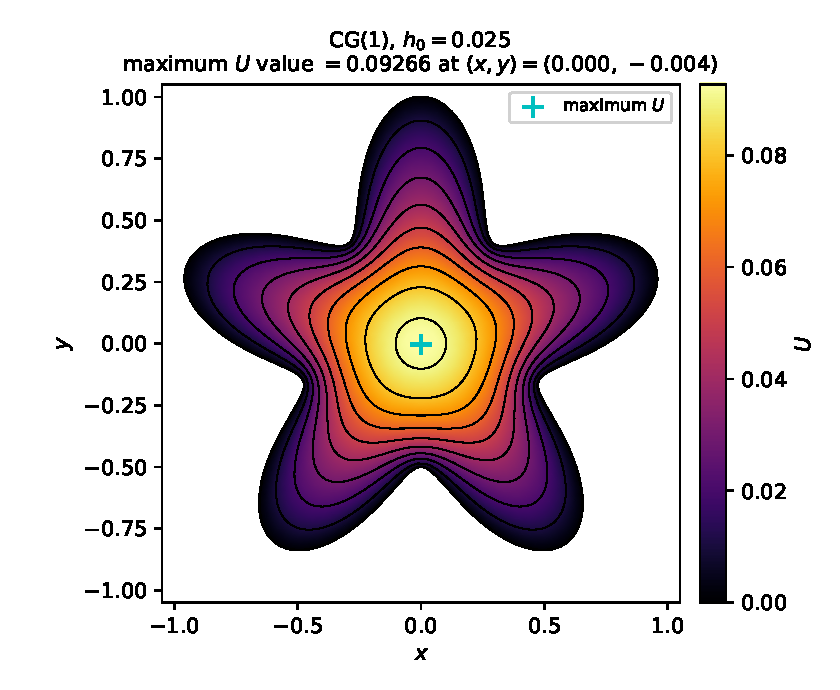
\includegraphics[width=0.5\linewidth]{hw4_p3_solution.pdf}
\captionof{figure}{CG(1) solution of $-\lap u=1$, $u=0$ on the star,
$h_{0}=0.025$ ($3167$ unknowns), with ten contours.  Cross: the largest nodal
value.}
\label{fig:p3}
\end{minipage}
\end{center}

\begin{center}
\begin{minipage}{\linewidth}
\centering\small
\begin{tabular}{@{}rrrcr@{}}
\toprule
$h_0$ & unknowns & $\max U$ & at $(x,y)$ & $\max U$, raw mesh\\
\midrule
0.100 & 149 & 0.09233 & $(0.000,\,0.032)$ & 0.23841\\
0.050 & 724 & 0.09256 & $(-0.026,\,-0.008)$ & 0.22573\\
0.025 & 3167 & 0.09266 & $(0.000,\,-0.004)$ & 0.22951\\
\bottomrule
\end{tabular}

\captionof{table}{The star under refinement.  ``Raw mesh'': the same nodes
without the fix \eqref{eq:snap} of Problem 2. None of these refinement ensure that center (0,0) get a node. It might be possible.}
\label{tab:p3}
\end{minipage}
\end{center}

The largest nodal value is $\max U=0.0927$.  It occurs at the node nearest
the centre, where the five-fold symmetry places it, and it is stable to three
digits from $h_{0}=0.05$ on.  Without the correction of Problem 2 the code
returns $\max U\approx0.23$.  The nodes missed in Problem 2 are then left
free, so along the valleys the code imposes no condition instead of $u=0$,
and the solution is wrong.\\

\textbf{Note:} on the raw mesh, \texttt{bnd2d} misses about half the boundary
nodes, all of them around the five valleys.  The solver treats those nodes as
unknowns, so nothing holds $u=0$ there.  What the missed nodes get instead: a
boundary node with no imposed value falls under the weak form's natural
condition, zero normal flux, $\partial u/\partial n=0$.  In membrane terms,
the rim is clamped only near the five tips and free along the valleys.

 

% ==================================================================
\problem{4(a)}{4a}

\textit{Recast this problem as a variational problem.  Clearly state the test
and trial function spaces.}

\medskip
The strong problem is
\begin{equation}\label{eq:pde}
  -\grad\cdot\grad u=-u_{,xx}-u_{,yy}=f(x,y)\quad\text{in } \Om=(-1,1)\times(-1,1),
  \qquad u=g\quad\text{on } \dOm .
\end{equation}

% ------------------------------------------------------------------
\subsection*{Multiplying by a test function and integrating by parts
  \ \src{product rule, then divergence theorem}}

Multiply \eqr{eq:pde} by a test function $v$ and integrate over $\Om$:
\begin{equation}\label{eq:mult}
  -\Iint v\,\lap u\dxdy=\Iint f v\dxdy .
\end{equation}
By the product rule, $\grad\cdot(v\grad u)=\grad v\cdot\grad u+v\,\lap u$, so
the left-hand side of \eqref{eq:mult} becomes
\begin{equation}\label{eq:prod}
  -\Iint v\,\lap u\dxdy=\Iint\grad u\cdot\grad v\dxdy-\Iint\grad\cdot(v\grad u)\dxdy .
\end{equation}
The divergence theorem, with $\nn$ the outward unit normal, turns the last
term into a boundary integral,
$\Iint\grad\cdot(v\grad u)\dxdy=\oint_{\dOm}v\,\grad u\cdot\nn\ds$.
Substituting this into \eqref{eq:prod}, and the result into \eqref{eq:mult},
gives
\begin{equation}\label{eq:ibp}
  \Iint\grad u\cdot\grad v\dxdy
  \;-\;\oint_{\dOm}v\,\underbrace{\grad u\cdot\nn}_{\text{normal flux, not given}}\ds
  \;=\;\Iint f v\dxdy .
\end{equation}

% ------------------------------------------------------------------
\subsection*{Removing the boundary term
  \ \src{Lecture 5: Dirichlet $=$ essential, the test function vanishes there}}

On all four sides the boundary data prescribe the \emph{value} $u=g$.  The
normal flux $\grad u\cdot\nn$ is therefore not known there; it is the
reaction needed to hold $u$ at $g$.  Consequently the boundary integral in
\eqr{eq:ibp} cannot be evaluated, and the only way to remove it is to require
$v=0$ on $\dOm$.  With that requirement, \eqr{eq:ibp} reduces to
\begin{equation}\label{eq:weak}
  \boxed{\;\Iint\grad u\cdot\grad v\dxdy=\Iint f v\dxdy\;}
\end{equation}

% ------------------------------------------------------------------
\subsection*{The trial set and the test space
  \ \src{from lecture : $u(0)=\alpha\neq0$ gives trial $\Vsp\neq$ test $\Vsp_{0}$;}} 

Equation \eqr{eq:weak} requires $\Iint\abs{\grad u}^{2}$ and
$\Iint\abs{\grad v}^{2}$ to be finite, so, from lecture, both spaces are
built on functions with $\Iint\bigl[v^{2}+\abs{\grad v}^{2}\bigr]\dxdy<\infty$.
In addition, the unknown $u$ must satisfy the essential condition $u=g$,
while the test function must vanish on the boundary.  This gives
\begin{equation}\label{eq:spaces}
  \boxed{\;
  \begin{aligned}
  \text{trial: }\ V_{g}&=\Bigl\{v:\ \Iint\bigl[v^{2}+\abs{\grad v}^{2}\bigr]\dxdy<\infty,
       \ \ v=g \text{ on } \dOm\Bigr\},\\
  \text{test: }\ V_{0}&=\Bigl\{v:\ \Iint\bigl[v^{2}+\abs{\grad v}^{2}\bigr]\dxdy<\infty,
       \ \ v=0 \text{ on } \dOm\Bigr\}=H^{1}_{0}(\Om),
  \end{aligned}\;}
\end{equation}
where $\abs{\grad v}^{2}=(v_{,x})^{2}+(v_{,y})^{2}$.  The two sets differ
because $g\neq0$ (in part (4.d), $g=1$).  This is a careful scenerio: $V_{g}$ is not a vector space, since the sum $u_{1}+u_{2}$ of two
of its members has boundary value $2g$, whereas $V_{0}$ is a vector space.

\medskip
\noindent\fbox{\parbox{0.955\linewidth}{%
\textbf{(Variational problem)}\ \ Find $u\in V_{g}$ such that
\[
  \Iint\grad u\cdot\grad v\dxdy=\Iint f v\dxdy
  \qquad\text{for all } v\in V_{0},
\]
with trial set $V_{g}$ and test space $V_{0}=H^{1}_{0}(\Om)$ from \eqr{eq:spaces}.}}

 

% ==================================================================
\newpage
\problem{4(b)}{4b}

\textit{Show that the variational problem has a unique solution by showing
that it meets all of the criteria of the Lax--Milgram theorem.}

% ------------------------------------------------------------------
\subsection*{Reduction to the form of the Lax--Milgram theorem
  \ \src{Lecture 13: $u$ and $v$ in the same Hilbert space;
         Lecture 5: lift the boundary data}}

The Lax--Milgram theorem of Lecture 13 requires a single Hilbert space $\Vsp$
that contains both $u$ and $v$.  In 4(a), however, $u\in V_{g}$ while
$v\in V_{0}$.  Lecture 5 resolves this by splitting off a known function that
carries the boundary data.

Let $G$ be any function in $V_{g}$.  (If $V_{g}$ were empty, there would be no
candidate $u$ at all.)  For part (d), where $g=1$, the constant $G\equiv1$
works, since $\Iint[1^{2}+0]\dxdy=4<\infty$.  Write $u=w+G$.  Then
$w=g-g=0$ on $\dOm$, so $w\in V_{0}$.  Substituting into \eqr{eq:weak} and
moving the known part to the right-hand side gives
\begin{equation}\label{eq:lifted}
  \underbrace{\Iint\grad w\cdot\grad v\dxdy}_{B(w,v)}
  \;=\;\underbrace{\Iint f v\dxdy-\Iint\grad G\cdot\grad v\dxdy}_{\widetilde{L}(v)}
  \qquad\forall\,v\in\Vsp:=V_{0}=H^{1}_{0}(\Om),
\end{equation}
where $\Vsp$ carries the norm of Lecture 13,
$\norm{v}^{2}_{\Vsp}=\norm{v}^{2}+\norm{\grad v}^{2}$, and $\norm{\cdot}$
denotes the $L^{2}(\Om)$ norm.

% ------------------------------------------------------------------
\subsection*{Symmetry (S) and continuity (CB)
  \ \src{Lecture 13, Part III, checks 1--2; Lecture 6: Cauchy}}

\textbf{(S)}\ \ Since $\grad w\cdot\grad v=\grad v\cdot\grad w$ at every
point, $B(w,v)=B(v,w)$.

\textbf{(CB)}\ \ The pointwise bound $\abs{\bm a\cdot\bm b}\le\abs{\bm a}\abs{\bm b}$,
the Cauchy inequality, and $\norm{\grad v}^{2}\le\norm{v}^{2}+\norm{\grad v}^{2}$
give in turn
\begin{equation}\label{eq:cb}
  \abs{B(w,v)}
  \le\underbrace{\Iint\abs{\grad w}\,\abs{\grad v}\dxdy}_{\abs{\bm a\cdot\bm b}\le\abs{\bm a}\abs{\bm b}}
  \le\underbrace{\norm{\grad w}\,\norm{\grad v}}_{\text{Cauchy}}
  \le\underbrace{\norm{w}_{\Vsp}\norm{v}_{\Vsp}}_{\norm{\grad v}^{2}\le\norm{v}^{2}+\norm{\grad v}^{2}},
  \qquad\beta^{*}=1 .
\end{equation}

% ------------------------------------------------------------------
\subsection*{Poincar\'e's inequality on the square
  \ \src{Lecture 8, eqs.~(1.127)--(1.128): the same three lines, in $x$, for
         each fixed $y$}}

Let $v\in V_{0}$ and fix $y$.  Since $v(-1,y)=0$ on the left side of the
square,
\begin{equation}\label{eq:p1}
  v(x,y)=\int_{-1}^{x}v_{,x}(s,y)\,\mathrm{d}s .
\end{equation}
Extending the integral to the whole line and applying the Cauchy inequality to
the product $1\cdot\abs{v_{,x}}$ on an interval of length $2$ gives
\begin{equation}\label{eq:p2}
  \abs{v(x,y)}\le\int_{-1}^{1}\abs{v_{,x}(s,y)}\,\mathrm{d}s
  \le\underbrace{\Bigl(\int_{-1}^{1}1^{2}\,\mathrm{d}s\Bigr)^{1/2}}_{\sqrt2}
     \Bigl(\int_{-1}^{1}v_{,x}(s,y)^{2}\,\mathrm{d}s\Bigr)^{1/2} .
\end{equation}
Now square \eqref{eq:p2}.  Its right-hand side no longer depends on $x$, so
integrating over $x\in(-1,1)$ multiplies it by $2$.  Integrating then over
$y\in(-1,1)$ gives
\begin{equation}\label{eq:poinc}
  \boxed{\;\norm{v}^{2}=\Iint v^{2}\dxdy\le
  \underbrace{2\cdot2}_{x\text{-length}\,\times\,\eqref{eq:p2}}\Iint(v_{,x})^{2}\dxdy
  \le4\,\norm{\grad v}^{2}\;}
\end{equation}
This is Lecture 13's multi-dimensional Poincar\'e inequality,
$\norm{v}\le C\norm{\grad v}$, with $C=2$.

% ------------------------------------------------------------------
\subsection*{Ellipticity (VE) and boundedness of $\widetilde{L}$
  \ \src{Lecture 13, Part III, checks 3--4}}

\textbf{(VE)}\ \ Split $B(v,v)$ into two halves and apply \eqr{eq:poinc} to
one of them:
\begin{equation}\label{eq:ve}
  B(v,v)=\norm{\grad v}^{2}
  =\tfrac12\norm{\grad v}^{2}+\underbrace{\tfrac12\norm{\grad v}^{2}}_{\ge\,\frac18\norm{v}^{2}\ \text{by \eqr{eq:poinc}}}
  \ge\tfrac18\bigl(\norm{\grad v}^{2}+\norm{v}^{2}\bigr)
  =\tfrac18\norm{v}^{2}_{\Vsp},
  \qquad\beta_{*}=\tfrac18 .
\end{equation}
This agrees with Lecture 13's $\beta_{*}=\tfrac12\min(1/C^{2},1)$ for $C=2$.

\textbf{$\widetilde{L}$ bounded}\ \ Applying the Cauchy inequality to each
term of \eqr{eq:lifted} gives
\begin{equation}\label{eq:lb}
  \abs{\widetilde{L}(v)}\le\norm{f}\,\norm{v}+\norm{\grad G}\,\norm{\grad v}
  \le\bigl(\norm{f}+\norm{\grad G}\bigr)\norm{v}_{\Vsp} .
\end{equation}
This requires $\Iint f^{2}<\infty$.  In part (d), $f$ is continuous on the
closed square.  Since $e^{\sin\pi x\sin\pi y}\le e$ and the expression in
braces has absolute value at most $2+2+1+1=6$, we have $\abs{f}\le6\pi^{2}e$.
Moreover $\grad G=0$.

\begin{center}
\begin{minipage}{\linewidth}
\centering\small
\renewcommand{\arraystretch}{1.25}
\begin{tabular}{@{}llll@{}}
\toprule
condition & holds because & constant & equation\\
\midrule
(S)  symmetric          & $\grad w\cdot\grad v=\grad v\cdot\grad w$ & --- & Step 2\\
(CB) bounded            & Cauchy                                   & $\beta^{*}=1$ & \eqref{eq:cb}\\
(VE) $\Vsp$-elliptic    & Poincar\'e, $C=2$                        & $\beta_{*}=1/8$ & \eqref{eq:ve}\\
$\widetilde{L}$ bounded & Cauchy                                   & $\norm{f}+\norm{\grad G}$ & \eqref{eq:lb}\\
\bottomrule
\end{tabular}
\captionof{table}{The four Lax--Milgram conditions for \eqr{eq:lifted} on
$\Vsp=H^{1}_{0}\bigl((-1,1)^{2}\bigr)$.}
\label{tab:lm}
\end{minipage}
\end{center}

% ------------------------------------------------------------------
\subsection*{Conclusion, and uniqueness of $u$ itself}

Table~\ref{tab:lm} shows that every hypothesis of the Lax--Milgram theorem is
satisfied.  Hence \eqr{eq:lifted} has a unique solution $w\in V_{0}$, with
$\norm{w}_{\Vsp}\le\bigl(\norm{f}+\norm{\grad G}\bigr)/\beta_{*}
=8\bigl(\norm{f}+\norm{\grad G}\bigr)$, and $u=w+G\in V_{g}$ solves the
variational problem of 4(a).

The solution $u$ does not depend on the choice of $G$.  Suppose
$u_{1},u_{2}\in V_{g}$ both solve the problem.  Their difference
$d=u_{1}-u_{2}$ has boundary value $g-g=0$, so $d\in V_{0}$, and subtracting
the two variational equations gives $B(d,v)=0$ for all $v\in V_{0}$.
Choosing $v=d$ and using \eqr{eq:ve},
\begin{equation}\label{eq:uniq}
  \tfrac18\norm{d}^{2}_{\Vsp}\le B(d,d)=0
  \qquad\Longrightarrow\qquad d=0,\ \ u_{1}=u_{2}.
\end{equation}

\medskip
\noindent\fbox{\parbox{0.955\linewidth}{%
\textbf{Conclusion.}  With $u=w+G$, the problem for $w$ on $H^{1}_{0}(\Om)$
satisfies (S), (CB) with $\beta^{*}=1$, (VE) with $\beta_{*}=1/8$, and
$\widetilde{L}$ is bounded.  By Lax--Milgram the variational problem of 4(a)
has exactly one solution $u\in V_{g}$.}}

\medskip
{\small\color{black!60}\textbf{Mechanics reading.}  (VE) is ``no rigid-body
mode'': the rim is held, so a membrane cannot move without stretching.
\eqr{eq:poinc} is the 2D version of Lecture 8's ``pinned ends cannot move for
free'' --- held on the left side, a deflection is controlled by its slope.
$\beta^{*}/\beta_{*}=8$ is the constant that C\'ea's lemma will carry into the
error estimate of part (d).}

% ==================================================================
\newpage
\problem{4(c)}{4c}

\textit{Develop a finite element method for this problem based on square
elements.  On each element the solution on the four corners is interpolated
with $s(x,y)=\alpha_{1}+\alpha_{2}x+\alpha_{3}y+\alpha_{4}xy$.  Write out the
basis functions and explicitly write out the linear system (uniform grid,
same spacing in $x$ and $y$).}

% ------------------------------------------------------------------
\subsection*{Grid and elements}

The square is divided into $N\times N$ elements of side $h=2/N$, with nodes
$x_{i}=-1+ih$ and $y_{j}=-1+jh$, $i,j=0,\dots,N$.  The $(N-1)^{2}$ interior
nodes, $1\le i,j\le N-1$, carry the unknowns, and the boundary nodes carry the
known values $g(x_{i},y_{j})$.  The corners of the element
$\Om_{ij}=[x_{i},x_{i+1}]\times[y_{j},y_{j+1}]$ are numbered
counter-clockwise starting from $(x_{i},y_{j})$ (Figure~\ref{fig:element}).

% ------------------------------------------------------------------
\subsection*{The basis functions on one element
  \ \src{the same steps as the triangle, Problem 3, eq.~\eqref{eq:hatK}}}

On $\Om_{ij}$, let $\varphi_{p}$ be the hat function of corner $p$
($p=1,2,3,4$): it equals $1$ at corner $p$ and $0$ at the other three
corners.  It has the form of the given interpolant,
$\varphi_{p}(x,y)=\alpha_{1}+\alpha_{2}x+\alpha_{3}y+\alpha_{4}xy$, with four
coefficients, one per corner, whose values depend on $p$.  Evaluating it at the four corners gives four equations for its
coefficients:
\begin{equation}\label{eq:hatQ}
  \underbrace{\begin{bmatrix}
    1&x_{i}&y_{j}&x_{i}y_{j}\\
    1&x_{i+1}&y_{j}&x_{i+1}y_{j}\\
    1&x_{i+1}&y_{j+1}&x_{i+1}y_{j+1}\\
    1&x_{i}&y_{j+1}&x_{i}y_{j+1}\end{bmatrix}}_{\bm X}
  \begin{bmatrix}\alpha_{1}\\\alpha_{2}\\\alpha_{3}\\\alpha_{4}\end{bmatrix}
  =\begin{bmatrix}\delta_{p1}\\\delta_{p2}\\\delta_{p3}\\\delta_{p4}\end{bmatrix}.
\end{equation}
This is the triangle's system \eqref{eq:hatK} with one more corner and one
more column, $xy$.  Take $p=1$.  Subtracting rows in pairs and using
$x_{i+1}-x_{i}=y_{j+1}-y_{j}=h$ gives
\begin{equation}\label{eq:elimQ}
  \underbrace{h\,(\alpha_{2}+\alpha_{4}y_{j})=-1}_{\text{row 2}\,-\,\text{row 1}},\qquad
  \underbrace{h\,(\alpha_{2}+\alpha_{4}y_{j+1})=0}_{\text{row 3}\,-\,\text{row 4}},\qquad
  \underbrace{h\,(\alpha_{3}+\alpha_{4}x_{i})=-1}_{\text{row 4}\,-\,\text{row 1}} .
\end{equation}
The second equation minus the first gives $h^{2}\alpha_{4}=1$.  Then the
second gives $\alpha_{2}$, the third gives $\alpha_{3}$, and row 3 of
\eqref{eq:hatQ} gives $\alpha_{1}$:
\begin{gather*}
  \alpha_{4}=\frac{1}{h^{2}},\qquad
  \alpha_{2}=-\frac{y_{j+1}}{h^{2}},\qquad
  \alpha_{3}=-\frac{1}{h}-\frac{x_{i}}{h^{2}}=-\frac{x_{i+1}}{h^{2}},\\
  \alpha_{1}=-\alpha_{2}x_{i+1}-\alpha_{3}y_{j+1}-\alpha_{4}x_{i+1}y_{j+1}=\frac{x_{i+1}y_{j+1}}{h^{2}} .
\end{gather*}
Hence
$\varphi_{1}=\bigl(x_{i+1}y_{j+1}-y_{j+1}x-x_{i+1}y+xy\bigr)/h^{2}
=(x_{i+1}-x)(y_{j+1}-y)/h^{2}$.  Moving the $1$ to corner $p=2,3,4$ and
repeating the same subtractions gives the other three hat functions:
\begin{equation}\label{eq:hatsQ}
  \boxed{\begin{aligned}
    \varphi_{1}&=\frac{(x_{i+1}-x)(y_{j+1}-y)}{h^{2}}, &\qquad
    \varphi_{2}&=\frac{(x-x_{i})(y_{j+1}-y)}{h^{2}},\\[2pt]
    \varphi_{3}&=\frac{(x-x_{i})(y-y_{j})}{h^{2}}, &\qquad
    \varphi_{4}&=\frac{(x_{i+1}-x)(y-y_{j})}{h^{2}}
  \end{aligned}}
\end{equation}
Each one has the form $\alpha_{1}+\alpha_{2}x+\alpha_{3}y+\alpha_{4}xy$, equals $1$ at its own corner, and has a
factor that vanishes at each of the other three corners, so it satisfies
\eqref{eq:hatQ}.  The subtractions in \eqref{eq:elimQ} solve
\eqref{eq:hatQ} for any right-hand side, so $\bm X$ is invertible and the
four corner values $s_{1},\dots,s_{4}$ determine the interpolant uniquely:
$s=\sum_{p=1}^{4}s_{p}\varphi_{p}$.

\begin{center}
\begin{minipage}{\linewidth}
\centering
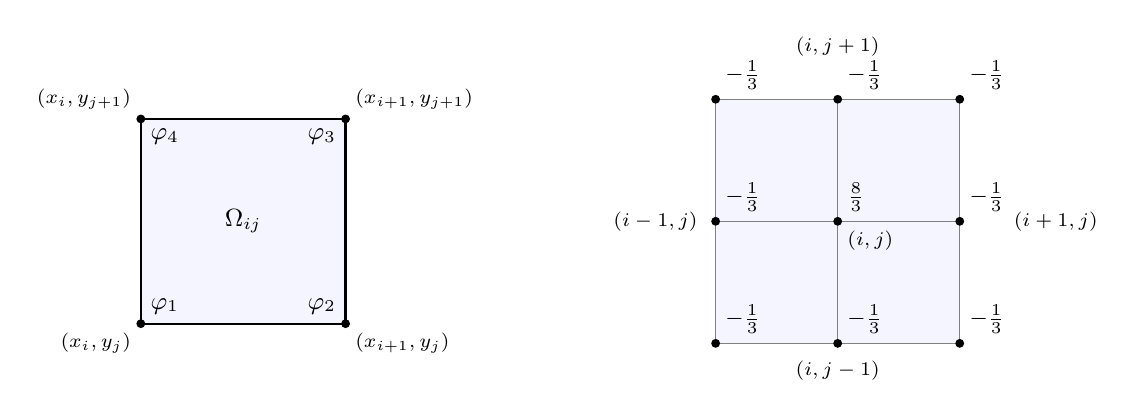
\begin{tikzpicture}[font=\small]
  % one element
  \begin{scope}[x=2.6cm,y=2.6cm]
    \draw[thick,fill=blue!4] (0,0) rectangle (1,1);
    \foreach \x/\y/\n/\pos in {0/0/1/above right,1/0/2/above left,1/1/3/below left,0/1/4/below right}
      {\fill (\x,\y) circle (1.6pt); \node[\pos] at (\x,\y) {$\varphi_{\n}$};}
    \node at (0.5,0.5) {$\Om_{ij}$};
    \node[font=\scriptsize,below left] at (0,0) {$(x_{i},y_{j})$};
    \node[font=\scriptsize,below right] at (1,0) {$(x_{i+1},y_{j})$};
    \node[font=\scriptsize,above right] at (1,1) {$(x_{i+1},y_{j+1})$};
    \node[font=\scriptsize,above left] at (0,1) {$(x_{i},y_{j+1})$};
  \end{scope}
  % the four elements around node (i,j)
  \begin{scope}[x=1.55cm,y=1.55cm,xshift=7.3cm,yshift=-0.25cm]
    \fill[blue!4] (0,0) rectangle (2,2);
    \foreach \t in {0,1,2}{\draw[gray] (\t,0) -- (\t,2); \draw[gray] (0,\t) -- (2,\t);}
    \foreach \x in {0,1,2}{\foreach \y in {0,1,2}{\fill (\x,\y) circle (1.6pt);}}
    \foreach \x/\y in {0/0,1/0,2/0,0/1,2/1,0/2,1/2,2/2}
      {\node[font=\footnotesize,above right=0pt] at (\x,\y) {$-\tfrac13$};}
    \node[font=\footnotesize,above right=0pt] at (1,1) {$\tfrac83$};
    \node[font=\scriptsize,below=3pt] at (1,0) {$(i,j-1)$};
    \node[font=\scriptsize,below right=0pt] at (1,1) {$(i,j)$};
    \node[font=\scriptsize,above=12pt] at (1,2) {$(i,j+1)$};
    \node[font=\scriptsize,left=3pt] at (0,1) {$(i-1,j)$};
    \node[font=\scriptsize,right=16pt] at (2,1) {$(i+1,j)$};
  \end{scope}
\end{tikzpicture}
\captionof{figure}{Left: one element $\Om_{ij}$ and the hat functions of its
corners, \eqr{eq:hatsQ}.  Right: the four elements around an interior node
$(i,j)$ --- the support of $\varphi_{ij}$ --- with the coefficients of its row
of the stiffness matrix, \eqr{eq:row}.}
\label{fig:element}
\end{minipage}
\end{center}

% ------------------------------------------------------------------
\subsection*{Continuity and the global basis
  \ \src{Lecture 3, eq.~(1.41): 1D hats; HW3 Problem 3: a jump puts a delta in
         the derivative}}

On the right edge of $\Om_{ij}$, where $x=x_{i+1}$, \eqref{eq:hatsQ} gives
$\varphi_{1}=\varphi_{4}=0$, so
$s=s_{2}(y_{j+1}-y)/h+s_{3}(y-y_{j})/h$, which is linear in $y$ and involves
only the two corner values on that edge.  The neighbouring element
$\Om_{i+1,j}$ produces the same linear function on its left edge from the
same two values.  Hence $s$ is continuous across every edge, $\grad s$
contains no delta function, and $\Iint\abs{\grad s}^{2}<\infty$.  The method
is therefore \textbf{conforming}: $V_{h}$ is contained in the spaces of
\eqr{eq:spaces}.

The global basis function of node $(i,j)$ is obtained by joining the hat
functions of the four squares around it (Figure~\ref{fig:element}, right).
The node is corner $1$ of $\Om_{ij}$, corner $2$ of $\Om_{i-1,j}$, corner $3$
of $\Om_{i-1,j-1}$ and corner $4$ of $\Om_{i,j-1}$.  On $\Om_{ij}$,
\eqref{eq:hatsQ} gives $(x_{i+1}-x)(y_{j+1}-y)/h^{2}$; on $\Om_{i-1,j}$ it
gives $(x-x_{i-1})(y_{j+1}-y)/h^{2}$; and similarly on the other two.  In
every case the $x$-factor, divided by $h$, is one half of Lecture 3's hat
function $\varphi_{i}$ on the $x$-grid, and the $y$-factor is one half of
$\varphi_{j}$ on the $y$-grid:
\begin{equation}\label{eq:basis}
  \boxed{\;\varphi_{ij}(x,y)=\varphi_{i}(x)\,\varphi_{j}(y),\qquad
  \varphi_{i}(x)=\begin{cases}
    (x-x_{i-1})/h, & x_{i-1}\le x\le x_{i},\\
    (x_{i+1}-x)/h, & x_{i}\le x\le x_{i+1},\\
    0, & \text{otherwise.}\end{cases}\;}
\end{equation}
The trial function carries the boundary values as Lecture 5's lift, and the
test functions are the interior basis functions:
\begin{equation}\label{eq:trial}
  U=\underbrace{\sum_{(k,l)\in\dOm}g(x_{k},y_{l})\,\varphi_{kl}}_{\text{known, carries }u=g}
   +\sum_{i,j=1}^{N-1}\xi_{ij}\,\varphi_{ij},
  \qquad v=\varphi_{ij},\ \ 1\le i,j\le N-1 .
\end{equation}

\medskip
\noindent\fbox{\parbox{0.955\linewidth}{%
\textbf{(FEM)}\ \ Find $U$ of the form \eqr{eq:trial} such that
$\displaystyle\Iint\grad U\cdot\grad\varphi_{ij}\dxdy=\Iint f\varphi_{ij}\dxdy$
for every interior node $(i,j)$.}}

% ------------------------------------------------------------------
\subsection*{The element stiffness matrix}

The gradient of $\varphi_{p}$ is the vector of its two partial derivatives,
$\grad\varphi_{p}=(\partial\varphi_{p}/\partial x,\,\partial\varphi_{p}/\partial y)$.
In each $\varphi_{p}$ of \eqref{eq:hatsQ}, $x$ appears in one factor and $y$
in the other, so $\partial/\partial x$ differentiates only the $x$-factor and
$\partial/\partial y$ only the $y$-factor.  For example, in
$\varphi_{1}=(x_{i+1}-x)(y_{j+1}-y)/h^{2}$, $\partial(x_{i+1}-x)/\partial x=-1$
gives $\partial\varphi_{1}/\partial x=-(y_{j+1}-y)/h^{2}$, and
$\partial(y_{j+1}-y)/\partial y=-1$ gives
$\partial\varphi_{1}/\partial y=-(x_{i+1}-x)/h^{2}$.  The four gradients on
$\Om_{ij}$ are
\begin{equation}\label{eq:gradQ}
  \begin{aligned}
  \grad\varphi_{1}&=\Bigl(\frac{\partial\varphi_{1}}{\partial x},\,\frac{\partial\varphi_{1}}{\partial y}\Bigr)=\Bigl(-\frac{y_{j+1}-y}{h^{2}},\;-\frac{x_{i+1}-x}{h^{2}}\Bigr),\\[3pt]
  \grad\varphi_{2}&=\Bigl(\frac{\partial\varphi_{2}}{\partial x},\,\frac{\partial\varphi_{2}}{\partial y}\Bigr)=\Bigl(\frac{y_{j+1}-y}{h^{2}},\;-\frac{x-x_{i}}{h^{2}}\Bigr),\\[3pt]
  \grad\varphi_{3}&=\Bigl(\frac{\partial\varphi_{3}}{\partial x},\,\frac{\partial\varphi_{3}}{\partial y}\Bigr)=\Bigl(\frac{y-y_{j}}{h^{2}},\;\frac{x-x_{i}}{h^{2}}\Bigr),\\[3pt]
  \grad\varphi_{4}&=\Bigl(\frac{\partial\varphi_{4}}{\partial x},\,\frac{\partial\varphi_{4}}{\partial y}\Bigr)=\Bigl(-\frac{y-y_{j}}{h^{2}},\;\frac{x_{i+1}-x}{h^{2}}\Bigr).
  \end{aligned}
\end{equation}
Unlike on the triangle, these are not constant, so the step ``a constant
leaves the integral'' of \eqref{eq:AK} is replaced by integration over
$\Om_{ij}$.  Each component in \eqref{eq:gradQ} depends on only one of $x$ and
$y$, so every integral separates into one-dimensional integrals over an
interval of length $h$:
\begin{equation}\label{eq:1d}
  \begin{gathered}
  \int_{x_{i}}^{x_{i+1}}\!\mathrm{d}x=h,\qquad
  \int_{x_{i}}^{x_{i+1}}\!(x_{i+1}-x)^{2}\,\mathrm{d}x
  =\int_{x_{i}}^{x_{i+1}}\!(x-x_{i})^{2}\,\mathrm{d}x=\frac{h^{3}}{3},\\
  \int_{x_{i}}^{x_{i+1}}\!\underbrace{(x_{i+1}-x)(x-x_{i})}_{h(x-x_{i})-(x-x_{i})^{2}}\mathrm{d}x
  =\frac{h^{3}}{2}-\frac{h^{3}}{3}=\frac{h^{3}}{6},
  \end{gathered}
\end{equation}
and the same in $y$.

The element stiffness matrix $\bm k^{e}$ is $4\times4$, one row and one
column per corner.  Its entry in row $p$ and column $q$, $p,q=1,2,3,4$, is
\begin{equation}\label{eq:kepq}
  k^{e}_{pq}=\iint_{\Om_{ij}}\grad\varphi_{p}\cdot\grad\varphi_{q}\dxdy ,
\end{equation}
the contribution of $\Om_{ij}$ to $A_{ji}$ in \eqref{eq:system3} when global
node $j$ is corner $p$ and global node $i$ is corner $q$.  Row $p$ is the
equation tested with $\varphi_{p}$; column $q$ multiplies the value of $U$ at
corner $q$.  For example, $k^{e}_{12}$ couples corner $1$ with corner $2$.
There are three kinds of pair: a corner with itself ($k^{e}_{11}$), two
corners that share an edge ($k^{e}_{12}$), and two opposite corners
($k^{e}_{13}$).  Each is computed from \eqref{eq:kepq} in the same steps.

\textbf{A corner with itself, $p=q=1$.}
\begin{align}
  k^{e}_{11}
  &=\iint_{\Om_{ij}}\grad\varphi_{1}\cdot\grad\varphi_{1}\dxdy
   &&\text{\eqref{eq:kepq} with }p=q=1\notag\\
  &=\iint_{\Om_{ij}}\Bigl(\frac{\partial\varphi_{1}}{\partial x},\,\frac{\partial\varphi_{1}}{\partial y}\Bigr)\cdot\Bigl(\frac{\partial\varphi_{1}}{\partial x},\,\frac{\partial\varphi_{1}}{\partial y}\Bigr)\dxdy
   &&\text{components of }\grad\notag\\
  &=\iint_{\Om_{ij}}\Bigl(\frac{\partial\varphi_{1}}{\partial x}\,\frac{\partial\varphi_{1}}{\partial x}+\frac{\partial\varphi_{1}}{\partial y}\,\frac{\partial\varphi_{1}}{\partial y}\Bigr)\dxdy
   &&\text{dot product}\notag\\
  &=\iint_{\Om_{ij}}\biggl(\Bigl[-\frac{y_{j+1}-y}{h^{2}}\Bigr]\Bigl[-\frac{y_{j+1}-y}{h^{2}}\Bigr]
   &&\text{by \eqref{eq:gradQ}}\notag\\
  &\qquad+\Bigl[-\frac{x_{i+1}-x}{h^{2}}\Bigr]\Bigl[-\frac{x_{i+1}-x}{h^{2}}\Bigr]\biggr)\dxdy\notag\\
  &=\frac{1}{h^{4}}\iint_{\Om_{ij}}\Bigl((y_{j+1}-y)^{2}+(x_{i+1}-x)^{2}\Bigr)\dxdy
   &&\text{multiply out}\notag\\
  &=\frac{1}{h^{4}}\Bigl[\int_{x_{i}}^{x_{i+1}}\!\!\mathrm{d}x\int_{y_{j}}^{y_{j+1}}\!\!(y_{j+1}-y)^{2}\mathrm{d}y
   &&\text{separate }x,\,y\notag\\
  &\qquad+\int_{x_{i}}^{x_{i+1}}\!\!(x_{i+1}-x)^{2}\mathrm{d}x\int_{y_{j}}^{y_{j+1}}\!\!\mathrm{d}y\Bigr]\notag\\
  &=\frac{1}{h^{4}}\Bigl[h\cdot\frac{h^{3}}{3}+\frac{h^{3}}{3}\cdot h\Bigr]
   &&\text{by \eqref{eq:1d}}\notag\\
  &=\frac13+\frac13=\frac46 .\label{eq:ke11}
\end{align}

\textbf{Two corners that share an edge, $p=1$, $q=2$.}
\begin{align}
  k^{e}_{12}
  &=\iint_{\Om_{ij}}\grad\varphi_{1}\cdot\grad\varphi_{2}\dxdy
   &&\text{\eqref{eq:kepq} with }p=1,\ q=2\notag\\
  &=\iint_{\Om_{ij}}\Bigl(\frac{\partial\varphi_{1}}{\partial x},\,\frac{\partial\varphi_{1}}{\partial y}\Bigr)\cdot\Bigl(\frac{\partial\varphi_{2}}{\partial x},\,\frac{\partial\varphi_{2}}{\partial y}\Bigr)\dxdy
   &&\text{components of }\grad\notag\\
  &=\iint_{\Om_{ij}}\Bigl(\frac{\partial\varphi_{1}}{\partial x}\,\frac{\partial\varphi_{2}}{\partial x}+\frac{\partial\varphi_{1}}{\partial y}\,\frac{\partial\varphi_{2}}{\partial y}\Bigr)\dxdy
   &&\text{dot product}\notag\\
  &=\iint_{\Om_{ij}}\biggl(\Bigl[-\frac{y_{j+1}-y}{h^{2}}\Bigr]\Bigl[\frac{y_{j+1}-y}{h^{2}}\Bigr]
   &&\text{by \eqref{eq:gradQ}}\notag\\
  &\qquad+\Bigl[-\frac{x_{i+1}-x}{h^{2}}\Bigr]\Bigl[-\frac{x-x_{i}}{h^{2}}\Bigr]\biggr)\dxdy\notag\\
  &=\frac{1}{h^{4}}\iint_{\Om_{ij}}\Bigl(-(y_{j+1}-y)^{2}+(x_{i+1}-x)(x-x_{i})\Bigr)\dxdy
   &&\text{multiply out}\notag\\
  &=\frac{1}{h^{4}}\Bigl[-\int_{x_{i}}^{x_{i+1}}\!\!\mathrm{d}x\int_{y_{j}}^{y_{j+1}}\!\!(y_{j+1}-y)^{2}\mathrm{d}y
   &&\text{separate }x,\,y\notag\\
  &\qquad+\int_{x_{i}}^{x_{i+1}}\!\!(x_{i+1}-x)(x-x_{i})\,\mathrm{d}x\int_{y_{j}}^{y_{j+1}}\!\!\mathrm{d}y\Bigr]\notag\\
  &=\frac{1}{h^{4}}\Bigl[-h\cdot\frac{h^{3}}{3}+\frac{h^{3}}{6}\cdot h\Bigr]
   &&\text{by \eqref{eq:1d}}\notag\\
  &=-\frac13+\frac16=-\frac16 .\label{eq:ke12}
\end{align}

\textbf{Two opposite corners, $p=1$, $q=3$.}
\begin{align}
  k^{e}_{13}
  &=\iint_{\Om_{ij}}\grad\varphi_{1}\cdot\grad\varphi_{3}\dxdy
   &&\text{\eqref{eq:kepq} with }p=1,\ q=3\notag\\
  &=\iint_{\Om_{ij}}\Bigl(\frac{\partial\varphi_{1}}{\partial x},\,\frac{\partial\varphi_{1}}{\partial y}\Bigr)\cdot\Bigl(\frac{\partial\varphi_{3}}{\partial x},\,\frac{\partial\varphi_{3}}{\partial y}\Bigr)\dxdy
   &&\text{components of }\grad\notag\\
  &=\iint_{\Om_{ij}}\Bigl(\frac{\partial\varphi_{1}}{\partial x}\,\frac{\partial\varphi_{3}}{\partial x}+\frac{\partial\varphi_{1}}{\partial y}\,\frac{\partial\varphi_{3}}{\partial y}\Bigr)\dxdy
   &&\text{dot product}\notag\\
  &=\iint_{\Om_{ij}}\biggl(\Bigl[-\frac{y_{j+1}-y}{h^{2}}\Bigr]\Bigl[\frac{y-y_{j}}{h^{2}}\Bigr]
   &&\text{by \eqref{eq:gradQ}}\notag\\
  &\qquad+\Bigl[-\frac{x_{i+1}-x}{h^{2}}\Bigr]\Bigl[\frac{x-x_{i}}{h^{2}}\Bigr]\biggr)\dxdy\notag\\
  &=\frac{1}{h^{4}}\iint_{\Om_{ij}}\Bigl(-(y_{j+1}-y)(y-y_{j})-(x_{i+1}-x)(x-x_{i})\Bigr)\dxdy
   &&\text{multiply out}\notag\\
  &=\frac{1}{h^{4}}\Bigl[-\int_{x_{i}}^{x_{i+1}}\!\!\mathrm{d}x\int_{y_{j}}^{y_{j+1}}\!\!(y_{j+1}-y)(y-y_{j})\,\mathrm{d}y
   &&\text{separate }x,\,y\notag\\
  &\qquad-\int_{x_{i}}^{x_{i+1}}\!\!(x_{i+1}-x)(x-x_{i})\,\mathrm{d}x\int_{y_{j}}^{y_{j+1}}\!\!\mathrm{d}y\Bigr]\notag\\
  &=\frac{1}{h^{4}}\Bigl[-h\cdot\frac{h^{3}}{6}-\frac{h^{3}}{6}\cdot h\Bigr]
   &&\text{by \eqref{eq:1d}}\notag\\
  &=-\frac16-\frac16=-\frac26 .\label{eq:kecases}
\end{align}
The factor $h^{4}$ cancels: in two dimensions the stiffness of a square
element does not depend on its size.  The matrix is symmetric,
$k^{e}_{pq}=k^{e}_{qp}$, and a quarter turn of the square maps corner
$1\to2\to3\to4\to1$, so every other entry repeats one of these three
values, and
\begin{equation}\label{eq:ke}
  \boxed{\;\bm{k}^{e}=\frac16\begin{bmatrix}
     4&-1&-2&-1\\ -1&4&-1&-2\\ -2&-1&4&-1\\ -1&-2&-1&4\end{bmatrix}\;}
\end{equation}
Each row sums to $0$, because a constant function has no gradient and
therefore no energy.

% ------------------------------------------------------------------
\subsection*{The linear system
  \ \src{Lecture 13, eq.~(1.236): $A_{ij}=B(\varphi_{i},\varphi_{j})$;
         Lecture 5, eq.~(1.66): known values to the RHS; Lecture 4: trapezoidal load}}

\textbf{Row of an interior node.}\ \ An interior node $(i,j)$ is a corner of
$4$ squares, shares each of its edge-neighbours with $2$ squares, and shares
each of its diagonal neighbours with $1$ square.  By \eqref{eq:ke11}--\eqref{eq:kecases}, its
diagonal entry is $4\cdot\tfrac46=\tfrac83$, an edge-neighbour entry is
$2\cdot(-\tfrac16)=-\tfrac13$, and a diagonal-neighbour entry is
$1\cdot(-\tfrac26)=-\tfrac13$; Figure~\ref{fig:assembly} carries out this
addition element by element.  The equation of node $(i,j)$ is therefore
\begin{equation}\label{eq:row}
  \boxed{\;\frac13\Bigl[\,8\,U_{i,j}-\sum_{(k,l)\in\mathcal{N}_{ij}}U_{k,l}\Bigr]=b_{ij},
  \qquad 1\le i,j\le N-1,\;}
\end{equation}
where $\mathcal{N}_{ij}$ is the set of eight neighbours $(k,l)$ with
$k\in\{i-1,i,i+1\}$, $l\in\{j-1,j,j+1\}$ and $(k,l)\neq(i,j)$, and
$U_{k,l}=g(x_{k},y_{l})$ whenever $(k,l)$ is a boundary node.

\textbf{Load vector.}\ \ The load entry is $b_{ij}=\Iint f\varphi_{ij}$.
Lecture 4's trapezoidal rule on each square,
$\iint_{\Om_{ij}}F\approx\tfrac{h^{2}}{4}\sum_{\text{corners}}F$, sees
$f\varphi_{ij}$ only at the corner $(i,j)$, where $\varphi_{ij}=1$.  Summing
over the four squares gives
\begin{equation}\label{eq:load}
  b_{ij}\approx4\cdot\tfrac{h^{2}}{4}\,f(x_{i},y_{j})=h^{2}f_{ij} .
\end{equation}

\textbf{Matrix form.}\ \ Order the unknowns row by row,
$\bm{U}=(U_{1,1},\dots,U_{N-1,1},\,U_{1,2},\dots,U_{N-1,N-1})^{T}$, and move
every boundary value in \eqr{eq:row} to the right-hand side.  The system
becomes
\begin{equation}\label{eq:system}
  \boxed{\begin{gathered}
  \bm{A}\,\bm{U}=\bm{b}+\bm{r},\qquad
  \bm{A}=\frac13\begin{bmatrix}
    \bm{T}&\bm{S}&&\\ \bm{S}&\bm{T}&\ddots&\\ &\ddots&\ddots&\bm{S}\\ &&\bm{S}&\bm{T}
  \end{bmatrix},\\[6pt]
  \bm{T}=\begin{bmatrix}8&-1&&\\-1&8&\ddots&\\&\ddots&\ddots&-1\\&&-1&8\end{bmatrix},\qquad
  \bm{S}=\begin{bmatrix}-1&-1&&\\-1&-1&\ddots&\\&\ddots&\ddots&-1\\&&-1&-1\end{bmatrix}
  \end{gathered}}
\end{equation}
Here $\bm{A}$ is $(N-1)^{2}\times(N-1)^{2}$ and consists of $N-1$ block rows.
The blocks $\bm{T}$ and $\bm{S}$ are $(N-1)\times(N-1)$: $\bm{T}$ couples a
node to its own grid row, and $\bm{S}$ couples it to the rows above and
below.  The boundary vector has entries $r_{ij}=\tfrac13\sum g(x_{k},y_{l})$,
summed over the boundary nodes among the eight neighbours of $(i,j)$.  For
$g=1$, as in part (d),
\begin{equation}\label{eq:r}
  r_{ij}=\begin{cases}
   5/3, & (i,j)\ \text{next to a corner (5 boundary neighbours)},\\
   1,   & (i,j)\ \text{next to one side (3 boundary neighbours)},\\
   0,   & \text{otherwise}.\end{cases}
\end{equation}
Finally, $\bm{A}$ is symmetric positive definite by Lecture 13's argument,
since (S) and (VE) of 4(b) hold whatever the element shape.
Figure~\ref{fig:assembly3} assembles \eqref{eq:system} and \eqref{eq:r}
square by square for $N=3$.

\medskip
{\small\color{black!60}\textbf{Same as finite differences?}  Divide
\eqr{eq:row} by $h^{2}$ and use \eqref{eq:load}:
$\bigl[8U_{i,j}-\sum_{\mathcal{N}_{ij}}U_{k,l}\bigr]/(3h^{2})=f_{ij}$, a
nine-point difference formula for $-\lap u$.  This is Lecture 4's ``CG(1) with
trapezoidal load is the central difference method'', one dimension up: the 2D
element couples diagonal neighbours too, which the five-point formula does
not.}

% ------------------------------------------------------------------
% Assembly of one row of A, element by element (Figure fig:assembly)
% generated layout; colours elone..elfour are defined in the preamble
\newpage
\begin{tcolorbox}[colback=white,colframe=black!55,boxrule=0.6pt,arc=2pt,
  left=5pt,right=5pt,top=2pt,bottom=1pt,colbacktitle=black!7,coltitle=black,
  title={\small\bfseries Assembly of row $(i,j)$ of $\bm A$\hfill
         \mdseries\src{Lecture 4, eq.~(1.56); Lecture 13, eq.~(1.236) and the array \texttt{t}}}]
\scriptsize
\begin{minipage}[c]{0.43\linewidth}\centering
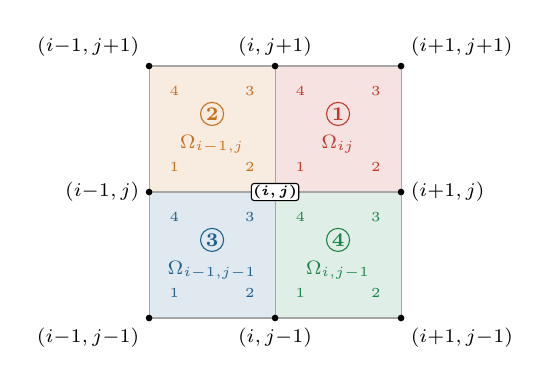
\begin{tikzpicture}[x=1.6cm,y=1.6cm,font=\scriptsize]
  \fill[elone!14]   (1,1) rectangle (2,2);
  \fill[eltwo!14]   (0,1) rectangle (1,2);
  \fill[elthree!14] (0,0) rectangle (1,1);
  \fill[elfour!14]  (1,0) rectangle (2,1);
  \foreach \t in {0,1,2}{\draw[gray!70] (\t,0) -- (\t,2); \draw[gray!70] (0,\t) -- (2,\t);}
  \foreach \a/\b/\n/\c/\name in {1/1/1/elone/{\Om_{ij}},0/1/2/eltwo/{\Om_{i-1,j}},
                                0/0/3/elthree/{\Om_{i-1,j-1}},1/0/4/elfour/{\Om_{i,j-1}}}{
    \node[circle,draw=\c,text=\c,inner sep=0.7pt,font=\scriptsize\bfseries] at (\a+0.5,\b+0.62) {\n};
    \node[text=\c] at (\a+0.5,\b+0.38) {$\name$};
    \node[text=\c,font=\tiny] at (\a+0.2,\b+0.2) {1};
    \node[text=\c,font=\tiny] at (\a+0.8,\b+0.2) {2};
    \node[text=\c,font=\tiny] at (\a+0.8,\b+0.8) {3};
    \node[text=\c,font=\tiny] at (\a+0.2,\b+0.8) {4};}
  \foreach \x in {0,1,2}{\foreach \y in {0,1,2}{\fill (\x,\y) circle (1.2pt);}}
  \node[below left]  at (0,0) {$(i{-}1,j{-}1)$};
  \node[below]       at (1,0) {$(i,j{-}1)$};
  \node[below right] at (2,0) {$(i{+}1,j{-}1)$};
  \node[left]        at (0,1) {$(i{-}1,j)$};
  \node[right]       at (2,1) {$(i{+}1,j)$};
  \node[above left]  at (0,2) {$(i{-}1,j{+}1)$};
  \node[above]       at (1,2) {$(i,j{+}1)$};
  \node[above right] at (2,2) {$(i{+}1,j{+}1)$};
  \node[fill=white,draw=black,rounded corners=1pt,inner sep=0.6pt,font=\tiny] at (1,1) {$\bm{(i,j)}$};
\end{tikzpicture}
\end{minipage}\hfill
\begin{minipage}[c]{0.55\linewidth}
\textbf{(a) The four squares around node $(i,j)$} (the right panel of
Figure~\ref{fig:element}).  The squares are numbered \en{1}{elone}--\en{4}{elfour}
counter-clockwise from $\Om_{ij}$.  Each square numbers its own corners $1$--$4$
(small numbers) counter-clockwise from its bottom-left corner, as in
\eqref{eq:hatsQ}, so node $(i,j)$ is corner $1$ of \en{1}{elone}, corner $2$ of
\en{2}{eltwo}, corner $3$ of \en{3}{elthree} and corner $4$ of \en{4}{elfour}.
The list of global nodes at corners $1$--$4$ of a square is its row of Lecture
13's connectivity array \texttt{t}.

\smallskip
\textbf{(b) The element matrix of each square} (below).  All four squares have
the same size and shape, so all four carry the same numbers, $\bm k^{e}$ of
\eqref{eq:ke}; only the names of the rows and columns differ.  Grey: local
corner numbers; under them, the global node at that corner.  Shaded: the row of
node $(i,j)$, the only row that enters row $(i,j)$ of $\bm A$.
\end{minipage}

\vspace{2pt}
\renewcommand{\arraystretch}{1.0}
\setlength{\tabcolsep}{4pt}
\begin{center}
\begin{tabular}{@{}c@{\hspace{3pt}}r|rrrr@{}}
\multicolumn{6}{@{}l}{\en{2}{eltwo}\ \textcolor{eltwo}{$\Om_{i-1,j}$}:\ \ $\bm k^{(2)}=\tfrac16\,\times$}\\[1pt]
 & & {\color{gray}1} & {\color{gray}2} & {\color{gray}3} & {\color{gray}4}\\
 & & $(i{-}1,j)$ & $(i,j)$ & $(i,j{+}1)$ & $(i{-}1,j{+}1)$\\\hline
{\color{gray}1} & $(i{-}1,j)$ & $4$ & $-1$ & $-2$ & $-1$\\
\rowcolor{eltwo!16}{\color{gray}2} & $(i,j)$ & $-1$ & $4$ & $-1$ & $-2$\\
{\color{gray}3} & $(i,j{+}1)$ & $-2$ & $-1$ & $4$ & $-1$\\
{\color{gray}4} & $(i{-}1,j{+}1)$ & $-1$ & $-2$ & $-1$ & $4$\\
\end{tabular}\hfill
\begin{tabular}{@{}c@{\hspace{3pt}}r|rrrr@{}}
\multicolumn{6}{@{}l}{\en{1}{elone}\ \textcolor{elone}{$\Om_{ij}$}:\ \ $\bm k^{(1)}=\tfrac16\,\times$}\\[1pt]
 & & {\color{gray}1} & {\color{gray}2} & {\color{gray}3} & {\color{gray}4}\\
 & & $(i,j)$ & $(i{+}1,j)$ & $(i{+}1,j{+}1)$ & $(i,j{+}1)$\\\hline
\rowcolor{elone!16}{\color{gray}1} & $(i,j)$ & $4$ & $-1$ & $-2$ & $-1$\\
{\color{gray}2} & $(i{+}1,j)$ & $-1$ & $4$ & $-1$ & $-2$\\
{\color{gray}3} & $(i{+}1,j{+}1)$ & $-2$ & $-1$ & $4$ & $-1$\\
{\color{gray}4} & $(i,j{+}1)$ & $-1$ & $-2$ & $-1$ & $4$\\
\end{tabular}\\[3pt]
\begin{tabular}{@{}c@{\hspace{3pt}}r|rrrr@{}}
\multicolumn{6}{@{}l}{\en{3}{elthree}\ \textcolor{elthree}{$\Om_{i-1,j-1}$}:\ \ $\bm k^{(3)}=\tfrac16\,\times$}\\[1pt]
 & & {\color{gray}1} & {\color{gray}2} & {\color{gray}3} & {\color{gray}4}\\
 & & $(i{-}1,j{-}1)$ & $(i,j{-}1)$ & $(i,j)$ & $(i{-}1,j)$\\\hline
{\color{gray}1} & $(i{-}1,j{-}1)$ & $4$ & $-1$ & $-2$ & $-1$\\
{\color{gray}2} & $(i,j{-}1)$ & $-1$ & $4$ & $-1$ & $-2$\\
\rowcolor{elthree!16}{\color{gray}3} & $(i,j)$ & $-2$ & $-1$ & $4$ & $-1$\\
{\color{gray}4} & $(i{-}1,j)$ & $-1$ & $-2$ & $-1$ & $4$\\
\end{tabular}\hfill
\begin{tabular}{@{}c@{\hspace{3pt}}r|rrrr@{}}
\multicolumn{6}{@{}l}{\en{4}{elfour}\ \textcolor{elfour}{$\Om_{i,j-1}$}:\ \ $\bm k^{(4)}=\tfrac16\,\times$}\\[1pt]
 & & {\color{gray}1} & {\color{gray}2} & {\color{gray}3} & {\color{gray}4}\\
 & & $(i,j{-}1)$ & $(i{+}1,j{-}1)$ & $(i{+}1,j)$ & $(i,j)$\\\hline
{\color{gray}1} & $(i,j{-}1)$ & $4$ & $-1$ & $-2$ & $-1$\\
{\color{gray}2} & $(i{+}1,j{-}1)$ & $-1$ & $4$ & $-1$ & $-2$\\
{\color{gray}3} & $(i{+}1,j)$ & $-2$ & $-1$ & $4$ & $-1$\\
\rowcolor{elfour!16}{\color{gray}4} & $(i,j)$ & $-1$ & $-2$ & $-1$ & $4$\\
\end{tabular}
\end{center}

\vspace{-2pt}
\textbf{(c) Adding the shaded rows.}  $A_{(i,j),(k,l)}=\Iint\grad\varphi_{kl}\cdot\grad\varphi_{ij}\dxdy$
is the sum of the integrals over the squares, so each shaded row goes into the
columns of its global nodes ($\cdot$: the square does not contain that node),
and each column adds what it received.

\smallskip
\begin{center}
\setlength{\tabcolsep}{3pt}
\begin{tabular}{@{}lccccccccc@{}}\toprule
column of $\bm A$ & $(i{-}1,j{-}1)$ & $(i,j{-}1)$ & $(i{+}1,j{-}1)$ & $(i{-}1,j)$ & $(i,j)$ & $(i{+}1,j)$ & $(i{-}1,j{+}1)$ & $(i,j{+}1)$ & $(i{+}1,j{+}1)$\\
{\color{gray}squares sharing both} & {\color{gray}1} & {\color{gray}2} & {\color{gray}1} & {\color{gray}2} & {\color{gray}4} & {\color{gray}2} & {\color{gray}1} & {\color{gray}2} & {\color{gray}1}\\\midrule
\en{1}{elone}\ shaded row of $\bm k^{(1)}$ & {\color{gray!60}$\cdot$} & {\color{gray!60}$\cdot$} & {\color{gray!60}$\cdot$} & {\color{gray!60}$\cdot$} & \textcolor{elone}{$4$} & \textcolor{elone}{$-1$} & {\color{gray!60}$\cdot$} & \textcolor{elone}{$-1$} & \textcolor{elone}{$-2$}\\
\en{2}{eltwo}\ shaded row of $\bm k^{(2)}$ & {\color{gray!60}$\cdot$} & {\color{gray!60}$\cdot$} & {\color{gray!60}$\cdot$} & \textcolor{eltwo}{$-1$} & \textcolor{eltwo}{$4$} & {\color{gray!60}$\cdot$} & \textcolor{eltwo}{$-2$} & \textcolor{eltwo}{$-1$} & {\color{gray!60}$\cdot$}\\
\en{3}{elthree}\ shaded row of $\bm k^{(3)}$ & \textcolor{elthree}{$-2$} & \textcolor{elthree}{$-1$} & {\color{gray!60}$\cdot$} & \textcolor{elthree}{$-1$} & \textcolor{elthree}{$4$} & {\color{gray!60}$\cdot$} & {\color{gray!60}$\cdot$} & {\color{gray!60}$\cdot$} & {\color{gray!60}$\cdot$}\\
\en{4}{elfour}\ shaded row of $\bm k^{(4)}$ & {\color{gray!60}$\cdot$} & \textcolor{elfour}{$-1$} & \textcolor{elfour}{$-2$} & {\color{gray!60}$\cdot$} & \textcolor{elfour}{$4$} & \textcolor{elfour}{$-1$} & {\color{gray!60}$\cdot$} & {\color{gray!60}$\cdot$} & {\color{gray!60}$\cdot$}\\
\midrule column sum & $\bm{-2}$ & $\bm{-2}$ & $\bm{-2}$ & $\bm{-2}$ & $\bm{16}$ & $\bm{-2}$ & $\bm{-2}$ & $\bm{-2}$ & $\bm{-2}$\\
$\times\tfrac16$ $=$ entry of $\bm A$ & $-\tfrac13$ & $-\tfrac13$ & $-\tfrac13$ & $-\tfrac13$ & {\boldmath$\tfrac83$} & $-\tfrac13$ & $-\tfrac13$ & $-\tfrac13$ & $-\tfrac13$\\\bottomrule
\end{tabular}
\end{center}
\vspace{-2pt}
An edge neighbour collects two $-1$'s (two squares share the edge), a diagonal
neighbour one $-2$ (one shared square), and the node itself four $4$'s.

\smallskip
\textbf{(d) The same addition in 1D: Lecture 4's bar.}  Two elements of
length $h$, both with $\bm k^{(1)}=\bm k^{(2)}=\tfrac1h\left[\begin{smallmatrix}1&-1\\-1&\phantom{-}1\end{smallmatrix}\right]$
(Lecture 4, eq.~(1.56), with $EA=1$).

\smallskip
\begin{minipage}[c]{0.49\linewidth}\centering
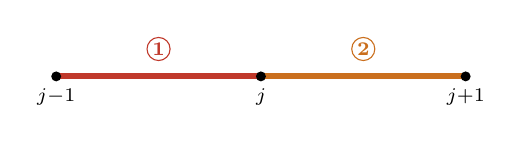
\begin{tikzpicture}[font=\scriptsize]
  \draw[line width=2.2pt,elone] (0,0) -- (2.6,0);
  \draw[line width=2.2pt,eltwo] (2.6,0) -- (5.2,0);
  \foreach \x/\l in {0/j{-}1,2.6/j,5.2/j{+}1}{\fill (\x,0) circle (1.8pt); \node[below=1pt] at (\x,0) {$\l$};}
  \node[above=2pt] at (1.3,0) {\en{1}{elone}};
  \node[above=2pt] at (3.9,0) {\en{2}{eltwo}};
\end{tikzpicture}

\smallskip
\begin{tabular}{@{}lccc@{}}\toprule
column of $\bm A$ & $j{-}1$ & $j$ & $j{+}1$\\\midrule
\en{1}{elone}\ row of $j$ (its corner $2$) & \textcolor{elone}{$-1$} & \textcolor{elone}{$1$} & {\color{gray!60}$\cdot$}\\
\en{2}{eltwo}\ row of $j$ (its corner $1$) & {\color{gray!60}$\cdot$} & \textcolor{eltwo}{$1$} & \textcolor{eltwo}{$-1$}\\\midrule
column sum $\times\tfrac1h$ $=$ entry of $\bm A$ & $-\tfrac1h$ & {\boldmath$\tfrac2h$} & $-\tfrac1h$\\\bottomrule
\end{tabular}
\end{minipage}\hfill
\begin{minipage}[c]{0.47\linewidth}
\begin{tabular}{@{}lll@{}}\toprule
 & 1D bar & 2D square\\\midrule
elements at the node & $2$ & $4$\\
diagonal & $2\times\tfrac1h$ & $4\times\tfrac46=\tfrac83$\\
neighbour in $2$ elements & --- & edge: $2\times(-\tfrac16)$\\
neighbour in $1$ element & $1\times(-\tfrac1h)$ & diagonal: $1\times(-\tfrac26)$\\
row sum & $0$ & $0$\\\bottomrule
\end{tabular}

\smallskip
\textbf{Mechanics.}  Each element acts as a spring between its nodes.  Every
element touching a node adds to that node's diagonal, and elements joining the
same two nodes act in parallel, so their stiffnesses add.  The bar's node $j$
hangs on two springs; the membrane's node $(i,j)$ on four squares.
\end{minipage}

\captionsetup{font=scriptsize,skip=3pt}
\captionof{figure}{Assembly of row $(i,j)$ of $\bm A$, \eqr{eq:row}, from
the four element matrices, and the same addition for Lecture~4's bar.}
\label{fig:assembly}
\end{tcolorbox}
% ------------------------------------------------------------------
% Assembly on a 3x3 patch (Figure fig:assembly3), generated layout;
% colours elone..elnine are defined in the preamble
\newpage
\begin{tcolorbox}[colback=white,colframe=black!55,boxrule=0.6pt,arc=2pt,
  left=5pt,right=5pt,top=2pt,bottom=1pt,colbacktitle=black!7,coltitle=black,
  title={\small\bfseries Assembly on a $3\times3$ patch\hfill
         \mdseries\src{Lecture 4, eq.~(1.56); Lecture 13, eq.~(1.236) and the array \texttt{t}}}]
\scriptsize
\textbf{(a) The patch.}  Figure~\ref{fig:assembly} with one more column ($i{+}2$)
and one more row ($j{+}2$); node $(i,j)$ is where it was, and squares
\en{1}{elone}--\en{4}{elfour} keep their numbers.  The new squares
\en{5}{elfive}--\en{9}{elnine} continue counter-clockwise.  Each node carries a
global number, as in \texttt{assemble.py}: the four inner nodes come first,
row by row ($\bm1=(i,j)$, $\bm2=(i{+}1,j)$, $\bm3=(i,j{+}1)$,
$\bm4=(i{+}1,j{+}1)$), then the outer ring $5$--$16$, counter-clockwise from
$(i{-}1,j{-}1)$.  Every square around an inner node lies in the patch, so the
rows of $\bm1$--$\bm4$ are complete.

\textbf{(b) The element matrix of each square}, placed where the square sits.
All nine carry the numbers of $\bm k^{e}$ in \eqref{eq:ke} (times $\tfrac16$),
with rows and columns in the order of corners $1$--$4$; the labels are the
global numbers at those corners, i.e.\ the square's row of \texttt{t}.
Shaded: rows of inner nodes, the ones assembled into $\bm A$.  A square
contributes one shaded row per inner node it touches: \en{1}{elone} four,
\en{2}{eltwo}\,\en{4}{elfour}\,\en{6}{elsix}\,\en{8}{eleight} two, and
\en{3}{elthree}\,\en{5}{elfive}\,\en{7}{elseven}\,\en{9}{elnine} one.

\smallskip
\begin{minipage}[c]{0.40\linewidth}\centering
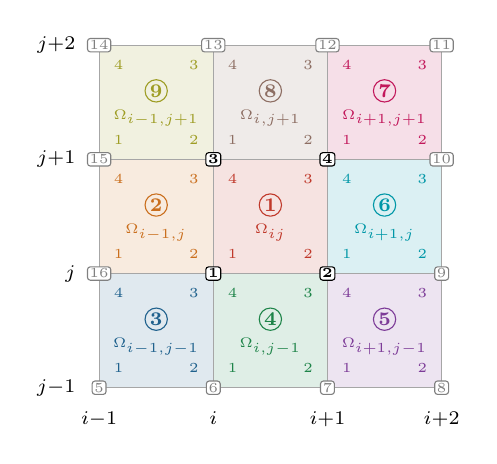
\begin{tikzpicture}[x=1.45cm,y=1.45cm,font=\scriptsize]
  \fill[elone!14] (1,1) rectangle (2,2);
  \fill[eltwo!14] (0,1) rectangle (1,2);
  \fill[elthree!14] (0,0) rectangle (1,1);
  \fill[elfour!14] (1,0) rectangle (2,1);
  \fill[elfive!14] (2,0) rectangle (3,1);
  \fill[elsix!14] (2,1) rectangle (3,2);
  \fill[elseven!14] (2,2) rectangle (3,3);
  \fill[eleight!14] (1,2) rectangle (2,3);
  \fill[elnine!14] (0,2) rectangle (1,3);
  \foreach \t in {0,1,2,3}{\draw[gray!70] (\t,0) -- (\t,3); \draw[gray!70] (0,\t) -- (3,\t);}
  \node[circle,draw=elone,text=elone,inner sep=0.6pt,font=\scriptsize\bfseries] at (1.5,1.6) {1};
  \node[text=elone,font=\tiny] at (1.5,1.36) {$\Om_{ij}$};
  \node[text=elone,font=\tiny] at (1.17,1.17) {1};
  \node[text=elone,font=\tiny] at (1.83,1.17) {2};
  \node[text=elone,font=\tiny] at (1.83,1.83) {3};
  \node[text=elone,font=\tiny] at (1.17,1.83) {4};
  \node[circle,draw=eltwo,text=eltwo,inner sep=0.6pt,font=\scriptsize\bfseries] at (0.5,1.6) {2};
  \node[text=eltwo,font=\tiny] at (0.5,1.36) {$\Om_{i-1,j}$};
  \node[text=eltwo,font=\tiny] at (0.17,1.17) {1};
  \node[text=eltwo,font=\tiny] at (0.83,1.17) {2};
  \node[text=eltwo,font=\tiny] at (0.83,1.83) {3};
  \node[text=eltwo,font=\tiny] at (0.17,1.83) {4};
  \node[circle,draw=elthree,text=elthree,inner sep=0.6pt,font=\scriptsize\bfseries] at (0.5,0.6) {3};
  \node[text=elthree,font=\tiny] at (0.5,0.36) {$\Om_{i-1,j-1}$};
  \node[text=elthree,font=\tiny] at (0.17,0.17) {1};
  \node[text=elthree,font=\tiny] at (0.83,0.17) {2};
  \node[text=elthree,font=\tiny] at (0.83,0.83) {3};
  \node[text=elthree,font=\tiny] at (0.17,0.83) {4};
  \node[circle,draw=elfour,text=elfour,inner sep=0.6pt,font=\scriptsize\bfseries] at (1.5,0.6) {4};
  \node[text=elfour,font=\tiny] at (1.5,0.36) {$\Om_{i,j-1}$};
  \node[text=elfour,font=\tiny] at (1.17,0.17) {1};
  \node[text=elfour,font=\tiny] at (1.83,0.17) {2};
  \node[text=elfour,font=\tiny] at (1.83,0.83) {3};
  \node[text=elfour,font=\tiny] at (1.17,0.83) {4};
  \node[circle,draw=elfive,text=elfive,inner sep=0.6pt,font=\scriptsize\bfseries] at (2.5,0.6) {5};
  \node[text=elfive,font=\tiny] at (2.5,0.36) {$\Om_{i+1,j-1}$};
  \node[text=elfive,font=\tiny] at (2.17,0.17) {1};
  \node[text=elfive,font=\tiny] at (2.83,0.17) {2};
  \node[text=elfive,font=\tiny] at (2.83,0.83) {3};
  \node[text=elfive,font=\tiny] at (2.17,0.83) {4};
  \node[circle,draw=elsix,text=elsix,inner sep=0.6pt,font=\scriptsize\bfseries] at (2.5,1.6) {6};
  \node[text=elsix,font=\tiny] at (2.5,1.36) {$\Om_{i+1,j}$};
  \node[text=elsix,font=\tiny] at (2.17,1.17) {1};
  \node[text=elsix,font=\tiny] at (2.83,1.17) {2};
  \node[text=elsix,font=\tiny] at (2.83,1.83) {3};
  \node[text=elsix,font=\tiny] at (2.17,1.83) {4};
  \node[circle,draw=elseven,text=elseven,inner sep=0.6pt,font=\scriptsize\bfseries] at (2.5,2.6) {7};
  \node[text=elseven,font=\tiny] at (2.5,2.36) {$\Om_{i+1,j+1}$};
  \node[text=elseven,font=\tiny] at (2.17,2.17) {1};
  \node[text=elseven,font=\tiny] at (2.83,2.17) {2};
  \node[text=elseven,font=\tiny] at (2.83,2.83) {3};
  \node[text=elseven,font=\tiny] at (2.17,2.83) {4};
  \node[circle,draw=eleight,text=eleight,inner sep=0.6pt,font=\scriptsize\bfseries] at (1.5,2.6) {8};
  \node[text=eleight,font=\tiny] at (1.5,2.36) {$\Om_{i,j+1}$};
  \node[text=eleight,font=\tiny] at (1.17,2.17) {1};
  \node[text=eleight,font=\tiny] at (1.83,2.17) {2};
  \node[text=eleight,font=\tiny] at (1.83,2.83) {3};
  \node[text=eleight,font=\tiny] at (1.17,2.83) {4};
  \node[circle,draw=elnine,text=elnine,inner sep=0.6pt,font=\scriptsize\bfseries] at (0.5,2.6) {9};
  \node[text=elnine,font=\tiny] at (0.5,2.36) {$\Om_{i-1,j+1}$};
  \node[text=elnine,font=\tiny] at (0.17,2.17) {1};
  \node[text=elnine,font=\tiny] at (0.83,2.17) {2};
  \node[text=elnine,font=\tiny] at (0.83,2.83) {3};
  \node[text=elnine,font=\tiny] at (0.17,2.83) {4};
  \node[fill=white,draw=black,rounded corners=1pt,inner sep=0.8pt,font=\tiny\bfseries] at (1,1) {1};
  \node[fill=white,draw=black,rounded corners=1pt,inner sep=0.8pt,font=\tiny\bfseries] at (2,1) {2};
  \node[fill=white,draw=black,rounded corners=1pt,inner sep=0.8pt,font=\tiny\bfseries] at (1,2) {3};
  \node[fill=white,draw=black,rounded corners=1pt,inner sep=0.8pt,font=\tiny\bfseries] at (2,2) {4};
  \node[fill=white,draw=gray,rounded corners=1pt,inner sep=0.8pt,font=\tiny,text=gray] at (0,0) {5};
  \node[fill=white,draw=gray,rounded corners=1pt,inner sep=0.8pt,font=\tiny,text=gray] at (1,0) {6};
  \node[fill=white,draw=gray,rounded corners=1pt,inner sep=0.8pt,font=\tiny,text=gray] at (2,0) {7};
  \node[fill=white,draw=gray,rounded corners=1pt,inner sep=0.8pt,font=\tiny,text=gray] at (3,0) {8};
  \node[fill=white,draw=gray,rounded corners=1pt,inner sep=0.8pt,font=\tiny,text=gray] at (3,1) {9};
  \node[fill=white,draw=gray,rounded corners=1pt,inner sep=0.8pt,font=\tiny,text=gray] at (3,2) {10};
  \node[fill=white,draw=gray,rounded corners=1pt,inner sep=0.8pt,font=\tiny,text=gray] at (3,3) {11};
  \node[fill=white,draw=gray,rounded corners=1pt,inner sep=0.8pt,font=\tiny,text=gray] at (2,3) {12};
  \node[fill=white,draw=gray,rounded corners=1pt,inner sep=0.8pt,font=\tiny,text=gray] at (1,3) {13};
  \node[fill=white,draw=gray,rounded corners=1pt,inner sep=0.8pt,font=\tiny,text=gray] at (0,3) {14};
  \node[fill=white,draw=gray,rounded corners=1pt,inner sep=0.8pt,font=\tiny,text=gray] at (0,2) {15};
  \node[fill=white,draw=gray,rounded corners=1pt,inner sep=0.8pt,font=\tiny,text=gray] at (0,1) {16};
  \node[below=5pt] at (0,0) {$i{-}1$};
  \node[below=5pt] at (1,0) {$i$};
  \node[below=5pt] at (2,0) {$i{+}1$};
  \node[below=5pt] at (3,0) {$i{+}2$};
  \node[left=5pt] at (0,0) {$j{-}1$};
  \node[left=5pt] at (0,1) {$j$};
  \node[left=5pt] at (0,2) {$j{+}1$};
  \node[left=5pt] at (0,3) {$j{+}2$};
\end{tikzpicture}
\end{minipage}\hfill
\begin{minipage}[c]{0.58\linewidth}\centering
\renewcommand{\arraystretch}{0.95}
\setlength{\tabcolsep}{2.2pt}
\begin{tabular}{@{}c@{\hspace{7pt}}c@{\hspace{7pt}}c@{}}
\begin{tabular}{@{}r|rrrr@{}}
\multicolumn{5}{@{}l@{}}{\en{9}{elnine}\,\textcolor{elnine}{$\Om_{i-1,j+1}$}}\\
 & {\color{gray}$15$} & $\bm{3}$ & {\color{gray}$13$} & {\color{gray}$14$}\\\hline
{\color{gray}$15$} & $4$ & $-1$ & $-2$ & $-1$\\
\rowcolor{elnine!16}$\bm{3}$ & $-1$ & $4$ & $-1$ & $-2$\\
{\color{gray}$13$} & $-2$ & $-1$ & $4$ & $-1$\\
{\color{gray}$14$} & $-1$ & $-2$ & $-1$ & $4$\\
\end{tabular}
&
\begin{tabular}{@{}r|rrrr@{}}
\multicolumn{5}{@{}l@{}}{\en{8}{eleight}\,\textcolor{eleight}{$\Om_{i,j+1}$}}\\
 & $\bm{3}$ & $\bm{4}$ & {\color{gray}$12$} & {\color{gray}$13$}\\\hline
\rowcolor{eleight!16}$\bm{3}$ & $4$ & $-1$ & $-2$ & $-1$\\
\rowcolor{eleight!16}$\bm{4}$ & $-1$ & $4$ & $-1$ & $-2$\\
{\color{gray}$12$} & $-2$ & $-1$ & $4$ & $-1$\\
{\color{gray}$13$} & $-1$ & $-2$ & $-1$ & $4$\\
\end{tabular}
&
\begin{tabular}{@{}r|rrrr@{}}
\multicolumn{5}{@{}l@{}}{\en{7}{elseven}\,\textcolor{elseven}{$\Om_{i+1,j+1}$}}\\
 & $\bm{4}$ & {\color{gray}$10$} & {\color{gray}$11$} & {\color{gray}$12$}\\\hline
\rowcolor{elseven!16}$\bm{4}$ & $4$ & $-1$ & $-2$ & $-1$\\
{\color{gray}$10$} & $-1$ & $4$ & $-1$ & $-2$\\
{\color{gray}$11$} & $-2$ & $-1$ & $4$ & $-1$\\
{\color{gray}$12$} & $-1$ & $-2$ & $-1$ & $4$\\
\end{tabular}\\[3pt]
\begin{tabular}{@{}r|rrrr@{}}
\multicolumn{5}{@{}l@{}}{\en{2}{eltwo}\,\textcolor{eltwo}{$\Om_{i-1,j}$}}\\
 & {\color{gray}$16$} & $\bm{1}$ & $\bm{3}$ & {\color{gray}$15$}\\\hline
{\color{gray}$16$} & $4$ & $-1$ & $-2$ & $-1$\\
\rowcolor{eltwo!16}$\bm{1}$ & $-1$ & $4$ & $-1$ & $-2$\\
\rowcolor{eltwo!16}$\bm{3}$ & $-2$ & $-1$ & $4$ & $-1$\\
{\color{gray}$15$} & $-1$ & $-2$ & $-1$ & $4$\\
\end{tabular}
&
\begin{tabular}{@{}r|rrrr@{}}
\multicolumn{5}{@{}l@{}}{\en{1}{elone}\,\textcolor{elone}{$\Om_{ij}$}}\\
 & $\bm{1}$ & $\bm{2}$ & $\bm{4}$ & $\bm{3}$\\\hline
\rowcolor{elone!16}$\bm{1}$ & $4$ & $-1$ & $-2$ & $-1$\\
\rowcolor{elone!16}$\bm{2}$ & $-1$ & $4$ & $-1$ & $-2$\\
\rowcolor{elone!16}$\bm{4}$ & $-2$ & $-1$ & $4$ & $-1$\\
\rowcolor{elone!16}$\bm{3}$ & $-1$ & $-2$ & $-1$ & $4$\\
\end{tabular}
&
\begin{tabular}{@{}r|rrrr@{}}
\multicolumn{5}{@{}l@{}}{\en{6}{elsix}\,\textcolor{elsix}{$\Om_{i+1,j}$}}\\
 & $\bm{2}$ & {\color{gray}$9$} & {\color{gray}$10$} & $\bm{4}$\\\hline
\rowcolor{elsix!16}$\bm{2}$ & $4$ & $-1$ & $-2$ & $-1$\\
{\color{gray}$9$} & $-1$ & $4$ & $-1$ & $-2$\\
{\color{gray}$10$} & $-2$ & $-1$ & $4$ & $-1$\\
\rowcolor{elsix!16}$\bm{4}$ & $-1$ & $-2$ & $-1$ & $4$\\
\end{tabular}\\[3pt]
\begin{tabular}{@{}r|rrrr@{}}
\multicolumn{5}{@{}l@{}}{\en{3}{elthree}\,\textcolor{elthree}{$\Om_{i-1,j-1}$}}\\
 & {\color{gray}$5$} & {\color{gray}$6$} & $\bm{1}$ & {\color{gray}$16$}\\\hline
{\color{gray}$5$} & $4$ & $-1$ & $-2$ & $-1$\\
{\color{gray}$6$} & $-1$ & $4$ & $-1$ & $-2$\\
\rowcolor{elthree!16}$\bm{1}$ & $-2$ & $-1$ & $4$ & $-1$\\
{\color{gray}$16$} & $-1$ & $-2$ & $-1$ & $4$\\
\end{tabular}
&
\begin{tabular}{@{}r|rrrr@{}}
\multicolumn{5}{@{}l@{}}{\en{4}{elfour}\,\textcolor{elfour}{$\Om_{i,j-1}$}}\\
 & {\color{gray}$6$} & {\color{gray}$7$} & $\bm{2}$ & $\bm{1}$\\\hline
{\color{gray}$6$} & $4$ & $-1$ & $-2$ & $-1$\\
{\color{gray}$7$} & $-1$ & $4$ & $-1$ & $-2$\\
\rowcolor{elfour!16}$\bm{2}$ & $-2$ & $-1$ & $4$ & $-1$\\
\rowcolor{elfour!16}$\bm{1}$ & $-1$ & $-2$ & $-1$ & $4$\\
\end{tabular}
&
\begin{tabular}{@{}r|rrrr@{}}
\multicolumn{5}{@{}l@{}}{\en{5}{elfive}\,\textcolor{elfive}{$\Om_{i+1,j-1}$}}\\
 & {\color{gray}$7$} & {\color{gray}$8$} & {\color{gray}$9$} & $\bm{2}$\\\hline
{\color{gray}$7$} & $4$ & $-1$ & $-2$ & $-1$\\
{\color{gray}$8$} & $-1$ & $4$ & $-1$ & $-2$\\
{\color{gray}$9$} & $-2$ & $-1$ & $4$ & $-1$\\
\rowcolor{elfive!16}$\bm{2}$ & $-1$ & $-2$ & $-1$ & $4$\\
\end{tabular}
\end{tabular}
\end{minipage}

\smallskip
\textbf{(c) Adding the shaded rows.}  Each shaded row is placed in row
$\bm p$ of $\bm A$ (its inner node) and in the columns of its global nodes; each
cell lists the contributions in the colour of the square they come from
($\cdot$: no square contains both nodes).

\smallskip
\begin{center}
\setlength{\tabcolsep}{1.45pt}
\begin{tabular}{@{}l|cccc|cccccccccccc@{}}\toprule
row$\,\backslash\,$node & $\bm{1}$ & $\bm{2}$ & $\bm{3}$ & $\bm{4}$ & {\color{gray}$5$} & {\color{gray}$6$} & {\color{gray}$7$} & {\color{gray}$8$} & {\color{gray}$9$} & {\color{gray}$10$} & {\color{gray}$11$} & {\color{gray}$12$} & {\color{gray}$13$} & {\color{gray}$14$} & {\color{gray}$15$} & {\color{gray}$16$}\\\midrule
$\bm{1}$ & ${\color{elone}4}{\color{eltwo}{+}4}{\color{elthree}{+}4}{\color{elfour}{+}4}$ & ${\color{elone}-1}{\color{elfour}{-}1}$ & ${\color{elone}-1}{\color{eltwo}{-}1}$ & ${\color{elone}-2}$ & ${\color{elthree}-2}$ & ${\color{elthree}-1}{\color{elfour}{-}1}$ & ${\color{elfour}-2}$ & {\color{gray!60}$\cdot$} & {\color{gray!60}$\cdot$} & {\color{gray!60}$\cdot$} & {\color{gray!60}$\cdot$} & {\color{gray!60}$\cdot$} & {\color{gray!60}$\cdot$} & {\color{gray!60}$\cdot$} & ${\color{eltwo}-2}$ & ${\color{eltwo}-1}{\color{elthree}{-}1}$\\
$\bm{2}$ & ${\color{elone}-1}{\color{elfour}{-}1}$ & ${\color{elone}4}{\color{elfour}{+}4}{\color{elfive}{+}4}{\color{elsix}{+}4}$ & ${\color{elone}-2}$ & ${\color{elone}-1}{\color{elsix}{-}1}$ & {\color{gray!60}$\cdot$} & ${\color{elfour}-2}$ & ${\color{elfour}-1}{\color{elfive}{-}1}$ & ${\color{elfive}-2}$ & ${\color{elfive}-1}{\color{elsix}{-}1}$ & ${\color{elsix}-2}$ & {\color{gray!60}$\cdot$} & {\color{gray!60}$\cdot$} & {\color{gray!60}$\cdot$} & {\color{gray!60}$\cdot$} & {\color{gray!60}$\cdot$} & {\color{gray!60}$\cdot$}\\
$\bm{3}$ & ${\color{elone}-1}{\color{eltwo}{-}1}$ & ${\color{elone}-2}$ & ${\color{elone}4}{\color{eltwo}{+}4}{\color{eleight}{+}4}{\color{elnine}{+}4}$ & ${\color{elone}-1}{\color{eleight}{-}1}$ & {\color{gray!60}$\cdot$} & {\color{gray!60}$\cdot$} & {\color{gray!60}$\cdot$} & {\color{gray!60}$\cdot$} & {\color{gray!60}$\cdot$} & {\color{gray!60}$\cdot$} & {\color{gray!60}$\cdot$} & ${\color{eleight}-2}$ & ${\color{eleight}-1}{\color{elnine}{-}1}$ & ${\color{elnine}-2}$ & ${\color{eltwo}-1}{\color{elnine}{-}1}$ & ${\color{eltwo}-2}$\\
$\bm{4}$ & ${\color{elone}-2}$ & ${\color{elone}-1}{\color{elsix}{-}1}$ & ${\color{elone}-1}{\color{eleight}{-}1}$ & ${\color{elone}4}{\color{elsix}{+}4}{\color{elseven}{+}4}{\color{eleight}{+}4}$ & {\color{gray!60}$\cdot$} & {\color{gray!60}$\cdot$} & {\color{gray!60}$\cdot$} & {\color{gray!60}$\cdot$} & ${\color{elsix}-2}$ & ${\color{elsix}-1}{\color{elseven}{-}1}$ & ${\color{elseven}-2}$ & ${\color{elseven}-1}{\color{eleight}{-}1}$ & ${\color{eleight}-2}$ & {\color{gray!60}$\cdot$} & {\color{gray!60}$\cdot$} & {\color{gray!60}$\cdot$}\\
\bottomrule\end{tabular}
\end{center}
\vspace{-2pt}
Times $\tfrac16$, every diagonal cell gives $\tfrac{16}{6}=\tfrac83$ and every
other filled cell $-\tfrac26=-\tfrac13$; each row sums to $0$.  The inner
columns $\bm1$--$\bm4$ form
\[
  \bm A=\frac13\begin{bmatrix}8&-1&-1&-1\\-1&8&-1&-1\\-1&-1&8&-1\\-1&-1&-1&8\end{bmatrix},
\]
and each row has five filled outer columns.  If the outer ring is $\dOm$ (the
grid $N=3$, $i=j=1$), those values $U=g$ move to the right-hand side as
$r=\tfrac13\sum g=\tfrac53$ for $g=1$: this is \eqref{eq:system} with
$\bm T=\left[\begin{smallmatrix}8&-1\\-1&8\end{smallmatrix}\right]$,
$\bm S=\left[\begin{smallmatrix}-1&-1\\-1&-1\end{smallmatrix}\right]$, and
\eqref{eq:r} for a node next to a corner.

\smallskip
\textbf{(d) The same in 1D: Lecture 4's bar with one more element.}  Node $j$
stays where it was; element \en{3}{elthree} is added on the right.  All three
have $\bm k^{e}=\tfrac1h\left[\begin{smallmatrix}1&-1\\-1&\phantom{-}1\end{smallmatrix}\right]$.

\smallskip
\begin{minipage}[c]{0.45\linewidth}\centering
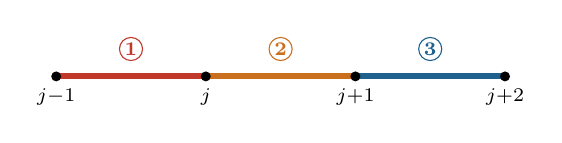
\begin{tikzpicture}[font=\scriptsize]
  \draw[line width=2.2pt,elone] (0,0) -- (1.9,0);
  \draw[line width=2.2pt,eltwo] (1.9,0) -- (3.8,0);
  \draw[line width=2.2pt,elthree] (3.8,0) -- (5.7,0);
  \foreach \x/\l in {0/j{-}1,1.9/j,3.8/j{+}1,5.7/j{+}2}{\fill (\x,0) circle (1.8pt); \node[below=1pt] at (\x,0) {$\l$};}
  \node[above=2pt] at (0.95,0) {\en{1}{elone}};
  \node[above=2pt] at (2.85,0) {\en{2}{eltwo}};
  \node[above=2pt] at (4.75,0) {\en{3}{elthree}};
\end{tikzpicture}
\end{minipage}\hfill
\begin{minipage}[c]{0.53\linewidth}\centering
\begin{tabular}{@{}l|cc|cc@{}}\toprule
row $\backslash$ node & $j$ & $j{+}1$ & $j{-}1$ & $j{+}2$\\\midrule
$j$     & ${\color{elone}1}{\color{eltwo}{+}1}$ & {\color{eltwo}$-1$} & {\color{elone}$-1$} & {\color{gray!60}$\cdot$}\\
$j{+}1$ & {\color{eltwo}$-1$} & ${\color{eltwo}1}{\color{elthree}{+}1}$ & {\color{gray!60}$\cdot$} & {\color{elthree}$-1$}\\\midrule
$\times\tfrac1h$ & \multicolumn{2}{c|}{$\tfrac1h\left[\begin{smallmatrix}2&-1\\-1&2\end{smallmatrix}\right]$} & \multicolumn{2}{c}{to the right-hand side}\\\bottomrule
\end{tabular}
\end{minipage}

\smallskip
The inner block is Lecture 4's matrix, eq.~(1.56), with two unknowns.
In both cases the rule is the same: a node's diagonal collects one term from
every element around it (two in 1D, four in 2D), and a pair of nodes collects
one term from every element that contains both.

\captionsetup{font=scriptsize,skip=3pt}
\captionof{figure}{Assembly on a $3\times3$ patch around node $(i,j)$: the
nine element matrices add up to the complete rows of the four inner nodes,
which for $N=3$ is the whole system \eqr{eq:system}.}
\label{fig:assembly3}
\end{tcolorbox}


\newpage
\problem{4(d)}{4d}

{\itshape Use the method of 4(c) to solve $-\grad\cdot\grad u=f$ on
$\Om=[-1,1]^{2}$, $u=g$ on $\dOm$, with
\[
  f=\pi^{2}e^{\sin(\pi x)\sin(\pi y)}\bigl\{2\sin(\pi x)\sin(\pi y)
   +2\cos^{2}(\pi x)\cos^{2}(\pi y)-\cos^{2}(\pi x)-\cos^{2}(\pi y)\bigr\},
  \qquad g=1 .
\]
Create a convergence table showing both $\norm{\cdot}_{V}$ and
$\norm{\cdot}_{L^{2}(\Om)}$ errors.  What order of convergence do you observe?
The exact solution is $u=e^{\sin(\pi x)\sin(\pi y)}$.\par}

\subsection*{Consistency of the data}

With $s=\sin\pi x\sin\pi y$ and $u=e^{s}$, we have
$u_{,x}=\pi\cos\pi x\sin\pi y\,e^{s}$, and differentiating once more in $x$
and in $y$ gives
\begin{align}
  -u_{,xx}-u_{,yy}
  &=\pi^{2}e^{s}\bigl[2\sin\pi x\sin\pi y
     -\cos^{2}\!\pi x\,\underbrace{\sin^{2}\!\pi y}_{1-\cos^{2}\pi y}
     -\underbrace{\sin^{2}\!\pi x}_{1-\cos^{2}\pi x}\cos^{2}\!\pi y\bigr]\notag\\
  &=\pi^{2}e^{s}\bigl[2\sin\pi x\sin\pi y+2\cos^{2}\!\pi x\cos^{2}\!\pi y
     -\cos^{2}\!\pi x-\cos^{2}\!\pi y\bigr]=f .\label{eq:lap}
\end{align}
This identity was also checked symbolically ($-\lap u-f\equiv0$).  On every
side of the square $\sin(\pm\pi)=0$, so $s=0$ and $u=e^{0}=1=g$.

\subsection*{Implementation \ \src{4(c); Lecture 4: trapezoidal rule; Lecture 5, eq.~(1.66)}}

The grids have $N\times N$ squares with $N=4,\dots,256$, so $h=2/N$ and there
are $(N-1)^{2}$ unknowns.  The stiffness matrix is assembled from the element
matrix $\bm k^{e}$ of 4(c), \eqref{eq:ke}, which is the same on every square,
as in Figures~\ref{fig:assembly} and~\ref{fig:assembly3}.  The code
checks that every interior row is the stencil $\tfrac13[8;\,-1\times8]$ of
4(c), that the interior matrix is symmetric positive definite, and that the
boundary terms are $5/3$, $1$ and $0$ as in 4(c).  The boundary values
$U=g=1$ are moved to the right-hand side, as in Lecture 5, so the code solves
\eqref{eq:system} with $\bm r$ of \eqref{eq:r}.

The load is the trapezoidal value $b_{ij}=h^{2}f_{ij}$ of 4(c),
\eqref{eq:load}.  The errors are measured in the norms of Lecture 13,
eq.~(1.254):
\begin{equation}\label{eq:norms}
  \norm{e}_{L^{2}(\Om)}^{2}=\iint_{\Om}(u-U)^{2}\dxdy,
  \qquad
  \norm{e}_{V}^{2}=\norm{e}_{L^{2}(\Om)}^{2}+\iint_{\Om}\abs{\grad(u-U)}^{2}\dxdy .
\end{equation}
These are integrals over the whole square, not nodal values.  The code
evaluates them in the following form.

\textbf{Trapezoidal rule on one square.}  Lecture 4's composite trapezoidal
rule on $[x_{i},x_{i+1}]$ with $M$ sub-intervals of length $h/M$ uses the
points $x_{i,a}=x_{i}+ah/M$, $a=0,\dots,M$, and the weights
\begin{equation}\label{eq:wtrap}
  w_{a}=\begin{cases}h/(2M), & a=0 \text{ or } a=M,\\ h/M, & 0<a<M.\end{cases}
\end{equation}
Applying it in $x$ and then in $y$ (points $y_{j,b}=y_{j}+bh/M$) gives, for any
$F$,
\begin{align}
  \iint_{\Om_{ij}}F\dxdy
  &=\int_{y_{j}}^{y_{j+1}}\Bigl(\int_{x_{i}}^{x_{i+1}}F\dx\Bigr)\mathrm{d}y
   &&\text{iterated integral}\notag\\
  &\approx\int_{y_{j}}^{y_{j+1}}\sum_{a=0}^{M}w_{a}F(x_{i,a},y)\,\mathrm{d}y
   &&\text{trapezoidal rule in } x\notag\\
  &\approx\sum_{a=0}^{M}\sum_{b=0}^{M}w_{a}w_{b}\,F(x_{i,a},y_{j,b})
   &&\text{trapezoidal rule in } y .\label{eq:trap2d}
\end{align}

\textbf{The $L^{2}$ error.}  On $\Om_{ij}$, $U=\sum_{p=1}^{4}U_{p}\varphi_{p}$,
where $U_{1},\dots,U_{4}$ are the values of $U$ at corners $1$--$4$ of
$\Om_{ij}$ and $\varphi_{p}$ are the hat functions \eqref{eq:hatsQ}.  Then
\begin{align}
  \norm{e}_{L^{2}(\Om)}^{2}
  &=\iint_{\Om}(u-U)^{2}\dxdy
   &&\text{by \eqref{eq:norms}}\notag\\
  &=\sum_{i,j=0}^{N-1}\iint_{\Om_{ij}}(u-U)^{2}\dxdy
   &&\Om\text{ is the union of the squares}\notag\\
  &=\sum_{i,j=0}^{N-1}\iint_{\Om_{ij}}\Bigl(u-\sum_{p=1}^{4}U_{p}\varphi_{p}\Bigr)^{2}\dxdy
   &&U\text{ on }\Om_{ij}\notag\\
  &\approx\sum_{i,j=0}^{N-1}\sum_{a,b=0}^{M}w_{a}w_{b}
     \Bigl(u-\sum_{p=1}^{4}U_{p}\varphi_{p}\Bigr)^{2}\Big|_{(x_{i,a},\,y_{j,b})}
   &&\text{by \eqref{eq:trap2d}} .\label{eq:eL2sum}
\end{align}

\textbf{The gradient part.}  With $\grad U=\sum_{p}U_{p}\grad\varphi_{p}$ and
the gradients \eqref{eq:gradQ},
\begin{align}
  \iint_{\Om}\abs{\grad(u-U)}^{2}\dxdy
  &=\sum_{i,j=0}^{N-1}\iint_{\Om_{ij}}\Bigl[\Bigl(\frac{\partial u}{\partial x}-\frac{\partial U}{\partial x}\Bigr)^{2}
     +\Bigl(\frac{\partial u}{\partial y}-\frac{\partial U}{\partial y}\Bigr)^{2}\Bigr]\dxdy
   &&\text{components of }\grad\notag\\
  &\approx\sum_{i,j=0}^{N-1}\sum_{a,b=0}^{M}w_{a}w_{b}
     \Bigl[\Bigl(\frac{\partial u}{\partial x}-\sum_{p=1}^{4}U_{p}\frac{\partial\varphi_{p}}{\partial x}\Bigr)^{2}
   &&\text{by \eqref{eq:gradQ}, \eqref{eq:trap2d}}\notag\\
  &\qquad\qquad+\Bigl(\frac{\partial u}{\partial y}-\sum_{p=1}^{4}U_{p}\frac{\partial\varphi_{p}}{\partial y}\Bigr)^{2}\Bigr]_{(x_{i,a},\,y_{j,b})} ,
   \label{eq:eH1sum}
\end{align}
where $\partial u/\partial x=\pi\cos\pi x\sin\pi y\,e^{s}$ and
$\partial u/\partial y=\pi\sin\pi x\cos\pi y\,e^{s}$ are the exact derivatives
from the consistency check above.  Finally, $\norm{e}_{V}^{2}$ is the sum of
\eqref{eq:eL2sum} and \eqref{eq:eH1sum}.

Equations \eqref{eq:eL2sum} and \eqref{eq:eH1sum} with $M=16$ are exactly what
\texttt{hw4\_p4d\_q1.py} computes; the code cites each equation it implements
by its number here.  (With $M=1$ the rule would use the corners only, that is,
nodal values only.)  Doubling the sub-grid from $M=8$ to $M=16$ changes the
errors by less than $2.5\%$ and leaves the rates unchanged.  The
observed rate is $\log_{2}\bigl(E(h)/E(h/2)\bigr)$, where $E$ is either
error.

\subsection*{Convergence table}

\begin{center}
\begin{minipage}{\linewidth}
\centering\small
\begin{tabular}{@{}rrrlclc@{}}
\toprule
$N$ & $h$ & unknowns & $\norm{e}_{V}$ & rate & $\norm{e}_{L^{2}(\Omega)}$ & rate\\
\midrule
4 & $0.50000$ & 9 & $2.1378\!\times\!10^{0}$ & --- & $2.3519\!\times\!10^{-1}$ & ---\\
8 & $0.25000$ & 49 & $1.4636\!\times\!10^{0}$ & 0.55 & $9.5737\!\times\!10^{-2}$ & 1.30\\
16 & $0.12500$ & 225 & $7.3914\!\times\!10^{-1}$ & 0.99 & $2.4256\!\times\!10^{-2}$ & 1.98\\
32 & $0.06250$ & 961 & $3.7048\!\times\!10^{-1}$ & 1.00 & $6.0808\!\times\!10^{-3}$ & 2.00\\
64 & $0.03125$ & 3969 & $1.8536\!\times\!10^{-1}$ & 1.00 & $1.5213\!\times\!10^{-3}$ & 2.00\\
128 & $0.01562$ & 16129 & $9.2693\!\times\!10^{-2}$ & 1.00 & $3.8038\!\times\!10^{-4}$ & 2.00\\
256 & $0.00781$ & 65025 & $4.6348\!\times\!10^{-2}$ & 1.00 & $9.5100\!\times\!10^{-5}$ & 2.00\\
\bottomrule
\end{tabular}

\captionof{table}{Bilinear squares on $[-1,1]^{2}$, $N\times N$ elements, trapezoidal load \eqr{eq:load}.}
\label{tab:p4d}
\end{minipage}
\end{center}

\begin{center}
\begin{minipage}{\linewidth}
\centering
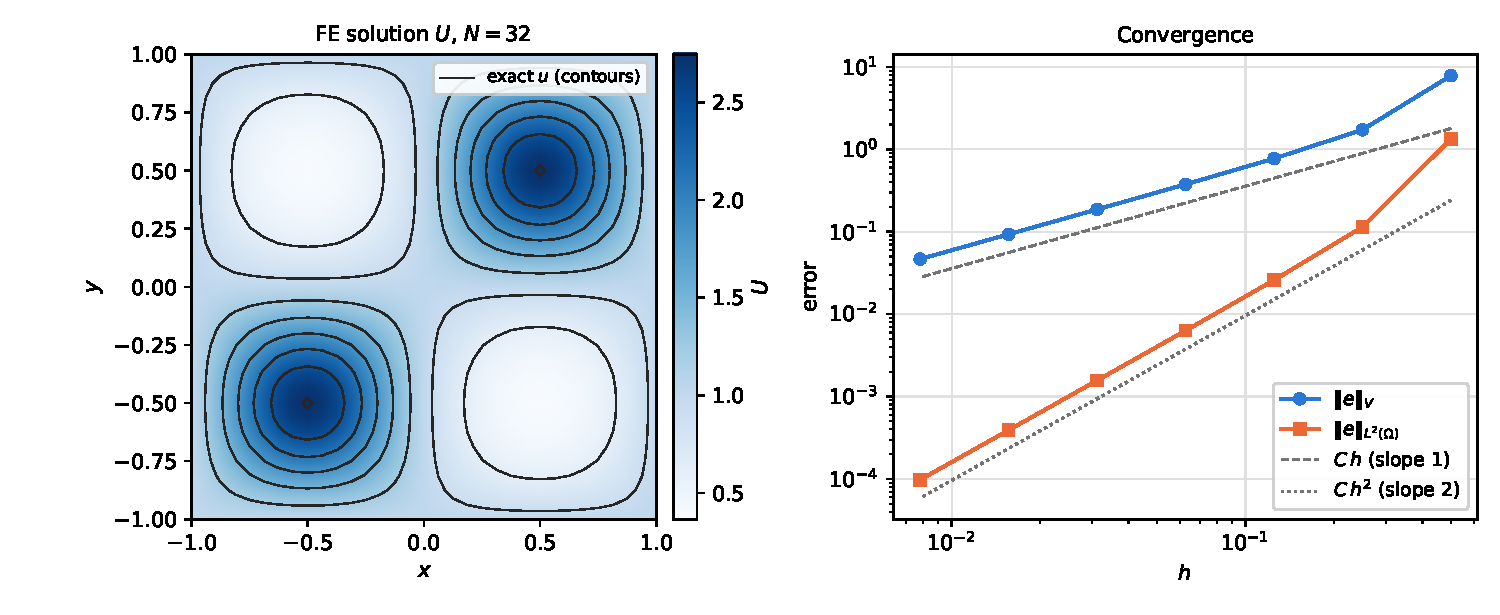
\includegraphics[width=\linewidth]{hw4_p4d_figure.pdf}
\captionof{figure}{Left: $U$ at $N=32$ with contours of the exact $u$.  Right:
the errors of Table~\ref{tab:p4d} against $h$, with slopes $1$ and $2$ for
reference.}
\label{fig:p4d}
\end{minipage}
\end{center}

\subsection*{The observed orders}

Table~\ref{tab:p4d} shows the rate in $\norm{e}_{V}$ tending to $1.00$, that
is, $\norm{e}_{V}=\mathcal O(h)$, and the rate in $\norm{e}_{L^{2}(\Om)}$
tending to $2.00$, that is, $\norm{e}_{L^{2}(\Om)}=\mathcal O(h^{2})$.  The
rates are clean from $N=32$ on.  At $N=4$ and $8$ the mesh has only two to four
squares across each bump of $u$, and the trapezoidal load samples $f$ at only
$9$ and $49$ interior nodes.

The first-order rate in $\norm{\cdot}_{V}$ follows from C\'ea's lemma.  The
boundary terms of 4(c) reproduce $g=1$ exactly, so $U-1$ is the Galerkin
approximation of $w=u-1\in H^{1}_{0}$, and C\'ea's lemma (Lecture 13,
eq.~(1.242)) with the constants of 4(b) gives
\begin{equation}\label{eq:cea}
  \norm{u-U}_{V}\le\frac{\beta^{*}}{\beta_{*}}\,\norm{u-v}_{V}
  =8\,\norm{u-v}_{V}\qquad\text{for every admissible } v\in V_{h} .
\end{equation}
Taking $v$ to be the bilinear interpolant of $u$ makes the right-hand side
$\mathcal O(h)$.  The second-order rate in $L^{2}$ follows from Lecture 7's
duality argument, in which the interpolation estimate is used twice, once for
$e$ and once for the dual solution, contributing one factor of $h$ each.

\outside{the interpolation estimate for squares}{Lecture 13 states
$\norm{u-u_{h}}_{H^{1}}\le c\,\norm{h\,u}_{H^{2}}$, eq.~(1.262), for linear
triangles.  The same $\mathcal O(h)$ bound for the bilinear interpolant on
squares, and the 2D duality argument behind $\mathcal O(h^{2})$ in $L^{2}$, are
standard but were not shown in class.  Table~\ref{tab:p4d} confirms both
rates.}

\medskip
\noindent\fbox{\parbox{0.955\linewidth}{%
\textbf{Conclusion.}  Bilinear squares converge at $\mathcal O(h)$ in
$\norm{\cdot}_{V}$ and $\mathcal O(h^{2})$ in $\norm{\cdot}_{L^{2}(\Om)}$ ---
the same orders as CG(1) --- with $\norm{e}_{V}=4.65\times10^{-2}$ and
$\norm{e}_{L^{2}}=9.78\times10^{-5}$ at $N=256$.}}

\end{document}
